\باب{طاقتی تسلسل، ٹیلر تسلسل اور لورنٹ تسلسل}
مخلوط تجزیہ میں طاقتی تسلسل (حصہ \حوالہ{حصہ_ٹیلر_طاقتی_تسلسل})  اہم ترین ہے چونکہ یہ تحلیلی تفاعل کو ظاہر کرتی ہے (مسئلہ \حوالہ{مسئلہ_ٹیلر_تحلیلی_تفاعل_تفرق})۔اسی طرح ہر تحلیلی تفاعل کا طاقتی تسلسل پایا جاتا ہے جس کو ٹیلر تسلسل کہتے ہیں۔یہ  ٹیلر تسلسل حقیقی علم الاحصاء کی ٹیلر تسلسل کی مخلوط مماثل ہیں۔بلکہ حقیقی ٹیلر تسلسل میں حقیقی متغیرہ کی جگہ مخلوط متغیرہ پر کرتے ہوئے ہم حقیقی تفاعل کو مخلوط دائرہ کار تک وسعت دے سکتے ہیں۔

باب کے آخری حصے میں تحلیلی تفاعل کی لورنٹ تسلسل پر غور کیا جائے گا۔ لورنٹ تسلسل میں غیر تابع متغیرہ کی مثبت اور منفی عدد صحیح طاقت پائے جاتے ہیں۔جیسا ہم اگلے باب میں دیکھیں گے، یہ تسلسل حقیقی اور مخلوط تکمل کی قیمت حاصل کرنے میں مدد گار ثابت ہوتی ہیں۔

%====================
\حصہ{طاقتی تسلسل}\شناخت{حصہ_ٹیلر_طاقتی_تسلسل}
گزشتہ باب کے حصہ \حوالہ{حصہ_ترتیب-تسلسل} میں مستقل اجزاء کی تسلسل کی تعریف پیش کی گئی۔اگر تسلسل کے اجزاء متغیر، مثلاً، متغیر \عددی{z} کے تفاعل  ہوں تب کسی مقررہ \عددی{z} کے لئے یہ تمام اجزاء کوئی مستقل ہوں گے لہٰذا وہ تمام تعریف یہاں بھی قابل استعمال ہوں گے۔ظاہر ہے کہ ایسا تسلسل جس کے اجزاء متغیر \عددی{z} کے تفاعل ہوں کے جزوی مجموعے، باقی اور مجموعہ بھی \عددی{z} کے تفاعل ہوں گے۔عموماً ایسا تسلسل \عددی{z} کی کچھ قیمتوں، مثلاً، کسی خطے میں تمام \عددی{z}  کے لئے مرتکز ہو گا، جبکہ \عددی{z} کی دیگر قیمتوں کے لئے تسلسل منفرج ہو گا۔ 

مخلوط تجزیہ میں متغیر اجزاء کی اہم ترین تسلسل طاقتی تسلسل ہے۔متغیر \عددی{z-a}  کی \اصطلاح{طاقتی تسلسل}\فرہنگ{طاقتی!تسلسل}\فرہنگ{تسلسل!طاقتی}\حاشیہب{power series}\فرہنگ{power!series}  درج ذیل روپ کی لامتناہی تسلسل کو کہتے ہیں
\begin{align}\label{مساوات_ٹیلر_طاقتی_تسلسل_الف}
\sum\limits_{m=0}^{\infty} c_m(z-a)^m=c_0+c_1(z-a)+c_2(z-a)^2+\cdots
\end{align}
 جہاں \عددی{z} کوئی متغیر ہے جبکہ \عددی{c_0,c_1,\cdots}، جنہیں \اصطلاح{عددی سر}\فرہنگ{عددی سر}\حاشیہب{coefficients}\فرہنگ{coefficients} کہتے ہیں، مستقل قیمتیں ہیں اور \عددی{a}، جس کو تسلسل کا \اصطلاح{مرکز}\فرہنگ{مرکز}\حاشیہب{center}\فرہنگ{center} کہتے ہیں، مستقل ہے۔طاقتی تسلسل  میں طاقت \عددی{m} صرف غیر منفی ہو سکتا ہے\حاشیہد{منفی \عددی{m} والے تسلسل پر اسی باب میں بعد میں غور کیا جائے گا۔}۔

\عددی{a=0} کی صورت میں طاقتی تسلسل کی درج ذیل مخصوص روپ حاصل ہوتی ہے جو \عددی{z} کی طاقتی تسلسل ہے۔
\begin{align}\label{مساوات_ٹیلر_طاقتی_تسلسل_ب}
\sum\limits_{m=0}^{\infty} c_mz^m=c_0+c_1z+c_2z^2+\cdots
\end{align}
 طاقتی تسلسل کی مرکوزیت کو سادہ طریقے سے بیان کیا جا سکتا ہے۔آئیں تین عمومی مثالوں سے شروع کرتے ہیں۔

%===================
\ابتدا{مثال}\شناخت{مثال_ٹیلر_قرص_میں_مرکوزیت}\quad \موٹا{قرص میں مرکوزیت، ہندسی تسلسل}\\
ہندسی تسلسل
\begin{align*}
\sum\limits_{m=0}^{\infty} z^m=1+z+z^2+\cdots
\end{align*}
\عددی{\abs{z}<1} کی صورت میں حتمی مرتکز جبکہ \عددی{\abs{z}\ge 1} کی صورت میں منفرج  ہے (مسئلہ \حوالہ{مسئلہ_ترتیب_ہندسی_تسلسل})۔
\انتہا{مثال}
%============================
\ابتدا{مثال}\شناخت{مثال_ٹیلر_پورے_متناہی_مستوی_میں_مرکوزیت}\quad \موٹا{پورے متناہی مستوی میں مرکوزیت}\\
درج ذیل طاقتی تسلسل
\begin{align*}
\sum\limits_{n=0}^{\infty} \frac{z^n}{n!}=1+z+\frac{z^2}{2!}+\frac{z^3}{3!}+\cdots
\end{align*}
تناسبی آزمائش کے تحت ہر (متناہی) \عددی{z} کے لئے حتمی مرتکز ہے۔در حقیقت کسی بھی مقررہ \عددی{z} کے لئے درج ذیل ہو گا۔
\begin{align*}
\abs{\frac{\tfrac{z^{n+1}}{(n+1)!}}{\tfrac{z^n}{n!}}}=\frac{\abs{z}}{n+1}\to 0 \quad \quad (n\to \infty)
\end{align*}
\انتہا{مثال}
%=====================
\ابتدا{مثال}\شناخت{مثال_ٹیلر_صرف_مرکز_پر_مرتکز}\quad \موٹا{صرف مرکز پر مرکوزیت}\\
درج ذیل تسلسل
\begin{align*}
\sum\limits_{n=0}^{\infty} n! z^n=1+z+2z^2+6z^3+\cdots
\end{align*}
صرف مرکز \عددی{z=0} پر مرتکز ہے جبکہ ہر \عددی{z\ne 0} کے لئے  تسلسل منفرج ہے۔یہی نتیجہ تناسبی آزمائش سے مقررہ \عددی{z} کے لئے حاصل کیا جا سکتا ہے یعنی:
\begin{align*}
\abs{\frac{(n+1)!z^{n+1}}{n!z^n}}=(n+1)\abs{z}\to \infty \quad \quad (n\to \infty,\quad z\ne 0)
\end{align*}
\انتہا{مثال}
%=======================

\عددی{z=a} کے لئے طاقتی تسلسل مساوات  \حوالہ{مساوات_ٹیلر_طاقتی_تسلسل_الف} مرتکز ہے چونکہ تب \عددی{z-a=0} ہو گا اور تسلسل واحد ایک جزو \عددی{c_0} پر مشتمل ہو گا۔ جیسا آپ نے مثال \حوالہ{مثال_ٹیلر_صرف_مرکز_پر_مرتکز} میں دیکھا، بعض اوقت \عددی{z} کی یہ واحد قیمت ہو گی جس پر تسلسل مرتکز ہو گا۔البتہ اگر تسلسل \حوالہ{مثال_ٹیلر_صرف_مرکز_پر_مرتکز} کسی \عددی{z_0\ne a} کے لئے مرتکز ہو تب تسلسل \عددی{z} کی ہر اس قیمت کے لئے مرتکز ہو گا  جس کا فاصلہ مرکز سے  \عددی{z_0} کے فاصلے سے کم ہو۔

%==================
\ابتدا{مسئلہ}\شناخت{مسئلہ_ٹیلر_طاقتی_تسلسل_کی_مرکوزیت}\quad \موٹا{طاقتی تسلسل کی مرکوزیت}\\
اگر مساوات \حوالہ{مساوات_ٹیلر_طاقتی_تسلسل_الف} میں دیا گیا طاقتی تسلسل نقطہ \عددی{z=a} پر مرتکز ہو تب یہ ہر اس \عددی{z} پر حتمی مرتکز ہو گا جس کے لئے
 \عددی{\abs{z-a}<\abs{z_0-a}} ہو، یعنی ایسے دائرے کے اندر ہر \عددی{z} پر جو \عددی{z_0} سے گزرتا ہو اور جس کا مرکز \عددی{a} ہو۔
\انتہا{مسئلہ}
%==================
\ابتدا{ثبوت}
چونکہ مساوات \حوالہ{مساوات_ٹیلر_طاقتی_تسلسل_الف} میں دیا گیا طاقتی تسلسل \عددی{z_0} پر مرتکز ہے لہٰذا مسئلہ \حوالہ{مسئلہ_ترتیب_مرکوزیت_شرط} کے تحت
\begin{align*}
c_n(z_0-a)^n\to 0 \quad \quad n\to \infty
\end{align*}
ہو گا یعنی \عددی{z=z_0} پر اس تسلسل کے اجزاء محدود ہوں گے، مثلاً ہر \عددی{n=0,1,2,\cdots} کے لئے
\begin{align*}
\abs{c_n(z_0-a)^n}<M\quad \quad \quad (n=0,1,2,\cdots)
\end{align*}
ہو گا۔اس سے  درج ذیل ملتا ہے
\begin{align*}
\abs{c_n(z_0-a)^n}=\abs{c_n(z_0-a)^n\big(\frac{z-a}{z_0-a}\big)^n}<M\abs{\frac{z-a}{z_0-a}}^n
\end{align*}
لہٰذا 
\begin{align}\label{مساوات_ٹیلر_ثبوت_طاقتی_تسلسل_مرکوزیت}
\sum\limits_{n=0}^{\infty}\abs{c_n(z_0-a)^n}<\sum\limits_{n=0}^{\infty}M\abs{\frac{z-a}{z_0-a}}^n=M\sum\limits_{n=0}^{\infty}\abs{\frac{z-a}{z_0-a}}^n
\end{align}
ہو گا۔چونکہ ہم فرض کر چکے ہیں کہ \عددی{\abs{z-a}<\abs{z_0-a}} لہٰذا
\begin{align*}
\abs{\frac{z-a}{z_0-a}}<1
\end{align*}
ہو گا اور یوں  مساوات \حوالہ{مساوات_ٹیلر_ثبوت_طاقتی_تسلسل_مرکوزیت} کی دائیں ہاتھ  (ہندسی) تسلسل مرتکز ہو گا۔یوں  مساوات \حوالہ{مساوات_ٹیلر_ثبوت_طاقتی_تسلسل_مرکوزیت} کا بایاں ہاتھ بھی مرتکز ہو گا لہٰذا مساوات \حوالہ{مساوات_ٹیلر_طاقتی_تسلسل_الف} میں دیا گیا تسلسل \عددی{\abs{z-a}<\abs{z_0-a}} کی صورت میں حتمی مرتکز ہو گا۔
\انتہا{ثبوت}
%====================

مثال \حوالہ{مثال_ٹیلر_پورے_متناہی_مستوی_میں_مرکوزیت} اور مثال \حوالہ{مثال_ٹیلر_صرف_مرکز_پر_مرتکز} میں ہم نے دیکھا کہ طاقتی تسلسل تمام \عددی{z} یا صرف \عددی{z=a} پر مرتکز ہو سکتا ہے۔آئیں ان دو صورتوں کو فی الحال نظر انداز کریں۔اب اگر کوئی  طاقتی تسلسل (مساوات \حوالہ{مساوات_ٹیلر_طاقتی_تسلسل_الف}) دیا گیا ہو تب ہم مخلوط مستوی میں ان تمام \عددی{z} پر غور کرتے ہیں جہاں تسلسل مرتکز ہو۔فرض کریں کہ \عددی{R} ایسا کم تر حقیقی عدد ہو کہ مرکز \عددی{a} سے ہر ایسے نقطے کا فاصلہ زیادہ سے زیادہ \عددی{R} ہو۔(مثال کے طور پر مثال \حوالہ{مثال_ٹیلر_قرص_میں_مرکوزیت} میں \عددی{R=1} ہے۔)  تب مسئلہ \حوالہ{مسئلہ_ٹیلر_طاقتی_تسلسل_کی_مرکوزیت} کے تحت رداس \عددی{R} کے دائرہ  جس کا مرکز \عددی{a} ہو میں تمام \عددی{z} پر تسلسل مرتکز ہو گا یعنی ان تمام \عددی{z} پر جو درج ذیل کو مطمئن کرتے ہوں
\begin{align}\label{مساوات_ٹیلر_رداس_مرکوزیت}
\abs{z-a}<R
\end{align}
اور \عددی{R} کی تعریف کے تحت ان تمام \عددی{z} پر جو 
\begin{align*}
\abs{z-a}>R
\end{align*}
کو مطمئن کرتے ہوں، تسلسل منفرج ہو گا۔دائرہ
\begin{align*}
\abs{z-a}=R
\end{align*}
کو \اصطلاح{دائرہ ارتکاز}\فرہنگ{ارتکاز!دائرہ}\فرہنگ{دائرہ!ارتکاز}\حاشیہب{convergence circle}\فرہنگ{convergence!circle} کہتے ہیں جبکہ \عددی{R} کو \اصطلاح{رداس ارتکاز}\فرہنگ{ارتکاز!رداس}\فرہنگ{رداس!ارتکاز}\حاشیہب{convergence radius}\فرہنگ{convergence!radius} کہتے ہیں (شکل \حوالہ{شکل_ٹیلر_دائرہ_مرکوزیت_رداس_مرکوزیت}-الف)۔
\begin{figure}
\centering
\begin{subfigure}{0.5\textwidth}
\centering
\begin{tikzpicture}
\draw(0,0)--++(2,0)node[right]{$x$};
\draw(0,0)--++(0,2)node[left]{$y$};
\draw(1,1) circle (0.75);
\draw[-stealth] (1,1)node[ocirc]{}node[left]{$a$}--++(30:0.75)node[pos=0.7,below]{$R$};
\end{tikzpicture}
\caption*{(الف) دائرہ ارتکاز}
\end{subfigure}%
\begin{subfigure}{0.5\textwidth}
\centering
\begin{tikzpicture}
\draw(-2,0)--(2,0)node[right]{$x$};
\draw[thick](-1,0)--(1,0);
\draw(-1,0)node[below]{$a-R$}--++(0,0.1);
\draw(1,0)node[below]{$a+R$}--++(0,0.1);
\draw(0,0)node[ocirc]{}node[below]{$a$};
\end{tikzpicture}
\caption*{(ب) حقیقی طاقتی تسلسل کا ارتکازی وقفہ}
\end{subfigure}%
\caption{دائرہ ارتکاز اور وقفہ ارتکاز}
\label{شکل_ٹیلر_دائرہ_مرکوزیت_رداس_مرکوزیت}
\end{figure}

دائرہ مرکوزیت کے نقطوں پر تسلسل مرتکز یا منفرج ہو سکتا ہے۔مثال کے طور پر مثال  \حوالہ{مثال_ٹیلر_قرص_میں_مرکوزیت} میں \عددی{R=1} ہے اور دائرہ مرکوزیت \عددی{\abs{z}=1} کے ہر نقطہ پر  تسلسل منفرج ہے۔طاقتی تسلسل
\begin{align*}
\sum\limits_{n=1}^{\infty} \frac{z^n}{n}=z+\frac{z^2}{2}+\frac{z^3}{3}+\cdots
\end{align*}
تناسبی آزمائش کے تحت \عددی{\abs{z}<1} پر مرتکز اور \عددی{\abs{z}>1} پر منفرج ہے۔عین \عددی{z=1} پر یہ ہارمونی تسلسل کی صورت اختیار کرتا ہے جو منفرج ہے جبکہ \عددی{z=-1} پر یہ \عددی{-1+\tfrac{1}{2}-\tfrac{1}{3}+\tfrac{1}{4}-+\cdots} صورت اختیار کرتا ہے جو مرتکز ہے (مثال \حوالہ{مثال_ترتیب_حتمی_اور_مشروط_مرکوز_تسلسل})۔آپ نے دیکھا کہ دائرہ مرکوزیت کے کچھ نقطوں پر تسلسل مرتکز اور کچھ نقطوں پر تسلسل منفرج ہو سکتا ہے۔

ظاہر ہے کہ اگر ہم حقیقی طاقتی تسلسل مساوات \حوالہ{مساوات_ٹیلر_طاقتی_تسلسل_الف} کی بات کی جائے جس کے عددی سر اور مرکز حقیقی ہوں اور  متغیرہ \عددی{z=x} ہو تب \عددی{x} محور پر  مساوات \حوالہ{مساوات_ٹیلر_رداس_مرکوزیت}  \اصطلاح{ارتکازی وقفہ}\فرہنگ{ارتکاز!وقفہ}\حاشیہب{interval of convergence}\فرہنگ{interval!of convergence} کو ظاہر کرے گا جس کی لمبائی \عددی{2R} اور درمیانہ نقطہ \عددی{x=a} ہو گا (شکل \حوالہ{شکل_ٹیلر_دائرہ_مرکوزیت_رداس_مرکوزیت}-ب)۔

اگر طاقتی تسلسل مساوات \حوالہ{مساوات_ٹیلر_طاقتی_تسلسل_الف} تمام \عددی{z} پر (مثال \حوالہ{مثال_ٹیلر_پورے_متناہی_مستوی_میں_مرکوزیت} کی طرح) مرتکز ہو تب ہم
\begin{align*}
R=\infty\quad \quad \text{اور}\quad \frac{1}{R}=0
\end{align*} 
لکھتے ہیں اور اگر تسلسل (مثال \حوالہ{مثال_ٹیلر_صرف_مرکز_پر_مرتکز} کی طرح) صرف مرکز \عددی{z=a} پر مرتکز ہو تب ہم
\begin{align*}
R=0\quad \quad \text{اور}\quad \frac{1}{R}=\infty
\end{align*}
لکھتے ہیں۔ان روایات کو استعمال کرتے ہوئے ارتکاز کے رداس \عددی{R} کو تسلسل کی عددی سروں سے حاصل کیا جا سکتا ہے یعنی:

%==================
\ابتدا{مسئلہ}\شناخت{مسئلہ_ٹیلر_رداس_ارتکاز}\quad \موٹا{ارتکاز کا رداس}\\
اگر ترتیب
$\,\sqrt[\leftroot{-2}n]{\abs{c_n}},\,\, n=1,2,\cdots\,$
مرتکز ہو اور اس کا حد \عددی{L} ہو، تب طاقتی تسلسل (مساوات \حوالہ{مساوات_ٹیلر_طاقتی_تسلسل_الف}) کا رداس ارتکاز \عددی{R} درج ذیل ہو گا
\begin{align}\label{مساوات_ٹیلر_رداس_ارتکاز_الف}
R=\frac{1}{L}
\end{align}
جو \عددی{L=0} کی صورت میں \عددی{R=\infty} دے گا اور تسلسل  (مساوات \حوالہ{مساوات_ٹیلر_طاقتی_تسلسل_الف}) تمام \عددی{z} کے لئے مرتکز ہو گا۔

اگر یہ ترتیب مرکوز نہ ہو لیکن محدود ہو، تب
\begin{align}\label{مساوات_ٹیلر_رداس_ارتکاز_ب}
R=\frac{1}{l}
\end{align}
ہو گا جہاں  ترتیب کے تحدیدی نقطوں میں سب سے بڑا تحدیدی نقطہ \عددی{l} ہے۔ 

اگر یہ ترتیب غیر محدود ہو، تب \عددی{R=0} ہو گا اور تسلسل صرف \عددی{z=a} پر مرتکز ہو گا۔

مساوات \حوالہ{مساوات_ٹیلر_رداس_ارتکاز_ب}\حاشیہد{فرانسیسی ریاضی دان آگستن لوئی کوشی [1789-1857] اور جیکویس ادامغ [1865-1964]}\فرہنگ{کوشی!اور ادامغ کلیہ}\حاشیہب{Cauchy-Hadamard formula}\فرہنگ{Cauchy!Hadamard formula} کلیہ کوشی اور ادامغ کہلاتا ہے۔
\انتہا{مسئلہ}
%========================
\ابتدا{ثبوت}\quad
اگر
\begin{align*}
\lim_{n\to\infty} \sqrt[\leftroot{-2}n]{\abs{c_n}}=L\ne 0
\end{align*}
ہو تب
\begin{align*}
\lim_{n\to\infty} \sqrt[\leftroot{-2}n]{\abs{c_n(z-a)^n}}=\abs{z-a}\lim_{n\to \infty} \sqrt[\leftroot{-2}n]{\abs{c_n}}=\abs{z-a} L
\end{align*}
ہو گا۔چونکہ تسلسل (مساوات \حوالہ{مساوات_ٹیلر_طاقتی_تسلسل_الف}) کے اجزاء 
$\,w_n=c_n(z-a)^n\,$
ہیں لہٰذا جذری آزمائش (حصہ \حوالہ{حصہ_ترتیب_تسلسل_آزمائش}) کے تحت
\begin{align*}
\abs{z-a}<\frac{1}{L}=R\quad \text{یا}\quad \abs{z-a}L<1 
\end{align*}
کی صورت میں تسلسل حتمی مرتکز ہو گا جبکہ
\begin{align*}
\abs{z-a}>\frac{1}{L}=R\quad \text{یا}\quad \abs{z-a}L>1
\end{align*}
کی صورت میں تسلسل منفرج ہو گا۔اگر
\begin{align*}
\lim_{n\to\infty} \sqrt[\leftroot{-2}n]{\abs{c_n}}=L=0
\end{align*}
ہو تب حد کی تعریف کے تحت کسی بھی \عددی{\epsilon>0} مثلاً \عددی{\epsilon=\tfrac{1}{2\abs{z_1-a}}} کے لئے جہاں \عددی{z_1} مستقل ہے، ہم ایسا \عددی{N} تلاش کر سکتے ہیں کہ ہر \عددی{n>N} کے لئے درج ذیل ہو۔
\begin{align*}
\sqrt[\leftroot{-2}n]{\abs{c_n}}<\frac{1}{2\abs{z_1-a}}\quad \quad \quad (n>N\,\text{ہر})
\end{align*} 
اس سے ہمیں
\begin{align*}
\abs{c_n}<\frac{1}{(2\abs{z_1-a})^n} \quad \implies \quad \abs{c_n(z_1-a)^n}<\frac{1}{2^n}
\end{align*}
ملتا ہے۔اب چونکہ \عددی{\sum 2^{-n}} مرتکز ہے لہٰذا تقابلی آزمائش  (حصہ \حوالہ{حصہ_ترتیب_تسلسل_آزمائش}) کے تحت \عددی{z=z_1} کے لئے تسلسل (مساوات \حوالہ{مساوات_ٹیلر_طاقتی_تسلسل_الف}) حتمی مرتکز ہے۔چونکہ \عددی{z_1} اختیاری ہے لہٰذا تسلسل ہر \عددی{z} کے لئے حتمی مرتکز ہے۔یوں مساوات \حوالہ{مساوات_ٹیلر_رداس_ارتکاز_الف} کا ذکر کرنے والے فقرے کا ثبوت مکمل ہوتا ہے۔

ہم اب اس فقرے کو ثابت کرتے ہیں جو مساوات \حوالہ{مساوات_ٹیلر_رداس_ارتکاز_ب} کا ذکر کرتا ہے۔ مسئلہ بُلزانو وائشسٹراس \حوالہ{مسئلہ_ترتیب_بلزانو_وائشسٹراس} کے تحت \عددی{l} موجود ہو گا اور چونکہ
$\,\sqrt[\leftroot{-2}n]{\abs{c_n}}\ge 0\,$
ہے لہٰذا \عددی{l>0} ہو گا۔حد کی تعریف کے تحت کسی بھی دیے گئے \عددی{\epsilon>0} کے لئے \عددی{n} کی لامتناہی تعداد کے لئے درج ذیل ہو گا۔
\begin{align*}
l-\epsilon<\sqrt[\leftroot{-2}n]{\abs{c_n}}<l+\epsilon\quad \quad \quad \text{\RL{$\,n\,$ کی لامتناہی تعداد}}
\end{align*}
اس کو مثبت مقدار \عددی{\abs{z-a}} سے ضرب دینے سے عدم مساوات
\begin{align}\label{مساوات_ٹیلر_رداس_ارتکاز_پ}
\abs{z-a}(l-\epsilon)<\sqrt[\leftroot{-2}n]{\abs{c_n(z-a)^n}}
\end{align}
اور
\begin{align}\label{مساوات_ٹیلر_رداس_ارتکاز_ت}
\sqrt[\leftroot{-2}n]{\abs{c_n(z-a)^n}}<\abs{z-a}(l+\epsilon)<
\end{align}
حاصل ہوتی ہیں۔چونکہ \عددی{l} سب سے بڑا تحدیدی نقطہ ہے لہٰذا  عدم مساوات \حوالہ{مساوات_ٹیلر_رداس_ارتکاز_ت} کے دائیں ہاتھ سے بڑے اجزاء کی تعداد متناہی ہو گی اور یوں 
 کافی بڑے تمام \عددی{n}، مثلاً \عددی{n>N}، کے لئے بھی عدم مساوات \حوالہ{مساوات_ٹیلر_رداس_ارتکاز_ت} مطمئن ہو گی۔ہم ثابت کرتے ہیں کہ
\begin{align}\label{مساوات_ٹیلر_رداس_ارتکاز_ٹ}
\abs{z-a}<\frac{1}{l}
\end{align}
کے لئے طاقتی تسلسل (مساوات \حوالہ{مساوات_ٹیلر_طاقتی_تسلسل_الف}) کا ارتکاز  عدم مساوات \حوالہ{مساوات_ٹیلر_رداس_ارتکاز_ت} سے ثابت ہوتا ہے۔در حقیقت، اگر ہم درج ذیل منتخب کریں
\begin{align*}
\epsilon=\frac{1-l\abs{z-a}}{2\abs{z-a}}
\end{align*}
تب مساوات \حوالہ{مساوات_ٹیلر_رداس_ارتکاز_ٹ} کے تحت \عددی{\epsilon>0} ہو گا اور عدم مساوات \حوالہ{مساوات_ٹیلر_رداس_ارتکاز_ت} درج ذیل صورت اختیار کرتی ہے۔
\begin{align*}
\sqrt[\leftroot{-2}n]{\abs{c_n(z-a)^n}}<\frac{1+l\abs{z-a}}{2}\quad \quad (n>N)
\end{align*}
مساوات \حوالہ{مساوات_ٹیلر_رداس_ارتکاز_ٹ} سے ہم دیکھتے ہیں کہ دایاں ہاتھ اکائی سے کم ہے لہٰذا مسئلہ \حوالہ{مسئلہ_ترتیب_جذری_آزمائش_ب} کے تحت تسلسل مرتکز ہو گا۔اس کے برعکس اگر 
\begin{align*}
\abs{z-a}>\frac{1}{l}
\end{align*}
ہو تب
\begin{align*}
\epsilon=\frac{l\abs{z-a}-1}{2\abs{z-a}}
\end{align*}
منتخب کرتے ہوئے \عددی{\epsilon>0} حاصل ہو گا اور  عدم مساوات \حوالہ{مساوات_ٹیلر_رداس_ارتکاز_پ} درج ذیل صورت اختیار کرے گی۔
\begin{align*}
\sqrt[\leftroot{-2}n]{\abs{c_n(z-a)^n}}>\frac{\abs{z-a}l+1}{2}>1
\end{align*}
یوں جذری آزمائش کے تحت ان \عددی{z} کے لئے تسلسل منفرج ہو گا۔یوں اس فقرے کا ثبوت مکمل ہوتا ہے  جو مساوات \حوالہ{مساوات_ٹیلر_رداس_ارتکاز_ب} کا ذکر کرتی ہے۔

آخر میں اگر ترتیب 
$\,\sqrt[\leftroot{-2}n]{\abs{c_n}}\,$
غیر محدود ہو، تب، انفراج کی تعریف کے تحت، کسی بھی \عددی{K} کے لئے
\begin{align*}
\sqrt[\leftroot{-2}n]{\abs{c_n}}>K\quad\quad \text{\RL{$\,n\,$ کی لامتناہی تعداد کے لئے}}
\end{align*}
ہو گا۔ہم 
$\,K=\tfrac{1}{\abs{z-a}}\,$
منتخب کرتے ہیں جہاں \عددی{z\ne a} ہے اور یوں عدم مساوات درج ذیل صورت اختیار کرتی ہے
\begin{align*}
\sqrt[\leftroot{-2}n]{\abs{c_n}}>\frac{1}{\abs{z-a}} \quad \implies \quad \sqrt[\leftroot{-2}n]{\abs{c_n(z-a)^n}}>1
\end{align*}
لہٰذا مسئلہ \حوالہ{مسئلہ_ترتیب_جذری_آزمائش_ب} کے تحت تسلسل منفرج ہو گا۔یوں اس مسئلے کا ثبوت مکمل ہوتا ہے۔
\انتہا{ثبوت}
%===========================

ہم اب طاقتی تسلسل کے مجموعہ اور ان کی تفریق پر غور کرتے ہیں۔

\ترچھا{دو طاقتی تسلسل کو جزو در جزو ان تمام \عددی{z} کے لئے جمع کیا جا سکتا ہے جن پر دونوں تسلسل مرتکز ہوں۔}  یہ نتیجہ مسئلہ \حوالہ{مسئلہ_ترتیب_مرتکز_تسلسلوں_کا_مجموعہ_مرتکز} سے اخذ ہوتا ہے۔

آئیں دو طاقتی تسلسل 
\begin{align}\label{مساوات_ٹیلر_کوشی_حاصل_ضرب_الف}
\sum_{k=0}^{\infty} a_kz^k=a_0+a_1z+\cdots\quad \text{اور}\quad \sum_{m=0}^{\infty}c_mz^m=c_1+c_1z+\cdots
\end{align}
کی جزو در جزو ضرب پر غور کرتے ہیں۔بائیں تسلسل کی ہر جزو کو دائیں تسلسل  کی ہر جزو سے ضرب دے کر \عددی{z} کی ایک جیسی طاقتوں کو یکجا کرتے ہوئے
\begin{multline}\label{مساوات_ٹیلر_کوشی_حاصل_ضرب_ب}
a_0c_0+(a_0c_1+a_1c_0)z+(a_0c_2+a_1c_1+a_2c_0)z^2+\cdots\\
\sum\limits_{n=0}^{\infty} (a_0c_n+a_1c_{n-1}+\cdots+z_nc_0)z^n
\end{multline}
ملتا ہے۔اس کو مساوات \حوالہ{مساوات_ٹیلر_کوشی_حاصل_ضرب_الف} میں دی گئی تسلسلوں  کا \اصطلاح{کوشی حاصل ضرب}\فرہنگ{کوشی!حاصل ضرب}\حاشیہب{Cauchy product}\فرہنگ{Cauchy!product} کہتے ہیں۔

%====================
\ابتدا{مسئلہ}\شناخت{مسئلہ_ٹیلر_طاقتی_تسلسل_کا_کوشی_حاصل_ضرب}\quad \موٹا{طاقتی تسلسلوں کا کوشی حاصل ضرب}\\
مساوات \حوالہ{مساوات_ٹیلر_کوشی_حاصل_ضرب_الف} میں ہر ایک تسلسل کی دائرہ ارتکاز کے اندر ہر \عددی{z} کے لئے کوشی حاصل ضرب  (مساوات \حوالہ{مساوات_ٹیلر_کوشی_حاصل_ضرب_ب}) حتمی مرتکز ہو گا۔اگر ان تسلسلوں کے مجموعے بالترتیب \عددی{g(z)} اور \عددی{h(z)} ہوں تب کوشی حاصل ضرب کا مجموعہ درج ذیل ہو گا۔
\begin{align}\label{مساوات_ٹیلر_کوشی_حاصل_ضرب_پ}
s(z)=g(z)h(z)
\end{align}
\انتہا{مسئلہ}
%====================
\ابتدا{ثبوت}\quad
کوشی حاصل ضرب(مساوات \حوالہ{مساوات_ٹیلر_کوشی_حاصل_ضرب_ب}) کا عمومی جزو 
\begin{align*}
p_n=(a_0c_n+a_1c_{n-1}+\cdots+z_nc_0)z^n
\end{align*}
ہے۔اب عمومی تکونی عدم مساوات \حوالہ{مساوات_مخلوط_عدم_مساوات_ب} سے درج ذیل حاصل ہوتا ہے
\begin{align*}
\abs{p_0}+\abs{p_1}=\abs{a_0c_0}+\abs{(a_0c_1+a_1c_0)z}\le (\abs{a_0}+\abs{a_1z})(\abs{c_0}+\abs{c_1z}),\\
\abs{p_0}+\abs{p_1}+\abs{p_2}\le (\abs{a_0}+\abs{a_1z}+\abs{a_2z^2})(\abs{c_0}+\abs{c_1z}+\abs{c_2z^2}),
\end{align*}
جس کی تصدیق آپ دائیں ہاتھ ضرب حاصل کرتے ہوئے کر سکتے ہیں؛ اسی طرح درج ذیل عمومی عدم مساوات لکھی جا سکتی ہے۔
\begin{multline}\label{مساوات_ٹیلر_کوشی_حاصل_ضرب_ت}
\abs{p_0}+\abs{p_1}+\cdots+\abs{p_n}\\
\le (\abs{a_0}+\abs{a_1z}+\cdots+\abs{a_nz^n})(\abs{c_0}+\abs{c_1z}+\cdots+\abs{c_nz^n})
\end{multline} 
اگر  \عددی{z} مساوات \حوالہ{مساوات_ٹیلر_کوشی_حاصل_ضرب_الف} میں ہر ایک تسلسل کے دائرہ ارتکاز کے اندر پایا جاتا ہو، تب  عدم مساوات \حوالہ{مساوات_ٹیلر_کوشی_حاصل_ضرب_ت} کا دایاں ہاتھ محدود ہو گا لہٰذا جزوی مجموعوں کی ترتیب کا مجموعہ  \عددی{\abs{p_0}+\abs{p_1}+\cdots} بھی محدود ہو گا۔چونکہ \عددی{\abs{p_n}\ge 0} ہے لہٰذا یہ ترتیب یک سر بڑھتی ترتیب ہو گی اور  مسئلہ \حوالہ{مسئلہ_ترتیب_حقیقی_ترتیب_مرکوزیت}  کے تحت مرتکز ہو گا۔یوں یہ تسلسل مرتکز ہے اور حاصل ضرب تسلسل (مساوات \حوالہ{مساوات_ٹیلر_کوشی_حاصل_ضرب_ب}) حتمی مرتکز ہو گا۔ 

ہم اب مساوات \حوالہ{مساوات_ٹیلر_کوشی_حاصل_ضرب_پ} کو ثابت کرتے ہیں۔ ہم اس حقیقت کو برائے کار لاتے ہیں کہ مساوات \حوالہ{مساوات_ٹیلر_کوشی_حاصل_ضرب_ب} کی ہر ردوبدل ان \عددی{z} کے لئے حتمی مرتکز ہے اور اس کا مجموعہ مساوات \حوالہ{مساوات_ٹیلر_کوشی_حاصل_ضرب_پ} دیتی ہے (مسئلہ \حوالہ{مسئلہ_ترتیب_حتمی_مرتکز_تسلسل_کی_ردوبدل})۔ہم ان میں سے ایک مخصوص ردوبدل 
$\,p^*_0+p^*_1+\cdots\,$
پر غور کرتے ہیں جہاں \عددی{p^*_n} درج ذیل ہے۔
\begin{align*}
(a_nc_0+a_0c_n)z^n+(a_nc_1+a_1c_n)z^{n+1}+\cdots+(a_nc_{n-1}+a_{n-1}c_n)z^{2n-1}+a_nc_nz^{2n}
\end{align*}
ظاہر ہے کہ 
\begin{align*}
a_0c_0=p^*_0,\quad (a_0+a_1z)(c_0+c_1z)=p^*_0+p^*_1
\end{align*}
اور عمومی جزو
\begin{align*}
(a_0+a_1z+\cdots+a_nz^n)(c_0+c_1z+\cdots+c_nz^n)=p^*_0+p^*_1+\cdots p^*_n
\end{align*}
ہیں۔اب \عددی{n} کو لامتناہی تک پہنچانے سے  مساوات \حوالہ{مساوات_ٹیلر_کوشی_حاصل_ضرب_پ} حاصل ہوتی ہے۔یوں مسئلے کا ثبوت مکمل ہوتا ہے۔
\انتہا{ثبوت}
%=========================

\ابتدا{مثال}\quad \موٹا{کوشی حاصل ضرب}\\
ہندسی تسلسل \عددی{1+z+z^2+\cdots} کا \عددی{\abs{z}<1} کی صورت میں مجموعہ \عددی{\tfrac{1}{1-z}} ہے (حصہ \حوالہ{حصہ_ترتیب_تسلسل_آزمائش})۔مسئلہ \حوالہ{مسئلہ_ٹیلر_طاقتی_تسلسل_کا_کوشی_حاصل_ضرب} سے درج ذیل حاصل ہو گا۔
\begin{align*}
\big(\frac{1}{1-z}\big)^2&=\sum\limits_{k=0}^{\infty} z^k\sum\limits_{m=0}^{\infty} z^m=(1+z+z^2+\cdots)(1+z+z^2+\cdots)\\
&=1+2z+3z^2+\cdots=\sum\limits_{n=0}^{\infty}(n+1)z^n\quad \quad (\abs{z}<1)
\end{align*}
\انتہا{مثال}
%====================

\حصہء{سوالات}
%=====================
\ابتدا{سوال}\quad
اگر ترتیب \عددی{\abs{\tfrac{c_{n+1}}{c_n}}}، جہاں \عددی{n=1,2,\cdots} ہے، مرتکز ہو اور اس کا حد \عددی{L} ہو تب دکھائیں کہ طاقتی تسلسل (مساوات \حوالہ{مساوات_ٹیلر_طاقتی_تسلسل_الف}) کی ارتکاز کے دائرے کا رداس، \عددی{L>0} کی صورت میں \عددی{R=\tfrac{1}{L}}  ہو گا جبکہ \عددی{L=0} کی صورت میں \عددی{R=\infty} ہو گا۔
\انتہا{سوال}
%================
\ابتدا{سوال}\quad
اگر مساوات \حوالہ{مساوات_ٹیلر_طاقتی_تسلسل_ب} میں دی گئی تسلسل کی ارتکاز کا رداس (جو متناہی تصور  کیا گیا ہو)\عددی{R}  ہے، تب دکھائیں کہ \عددی{\sum c_mz^{2m}} کی ارتکاز کا رداس \عددی{\sqrt{R}} ہو گا۔
\انتہا{سوال}
%====================
سوال \حوالہ{سوال_ٹیلر_ارتکاز_کا_رداس_الف} تا سوال \حوالہ{سوال_ٹیلر_ارتکاز_کا_رداس_ب} میں ارتکاز کا رداس تلاش کریں۔

%======================
\ابتدا{سوال}\شناخت{سوال_ٹیلر_ارتکاز_کا_رداس_الف}\quad
$\sum\limits_{n=0}^{\infty} (z-i2)^n$\\
جواب:\quad
$1$
\انتہا{سوال}
%=============================
\ابتدا{سوال}\quad
$\sum\limits_{n=0}^{\infty} \tfrac{(z-2)^n}{2^n}$
\انتہا{سوال}
%=============================
\ابتدا{سوال}\quad
$\sum\limits_{n=0}^{\infty} n(\tfrac{z}{3})^n$\\
جواب:\quad
$3$
\انتہا{سوال}
%=============================
\ابتدا{سوال}\quad
$\sum\limits_{n=0}^{\infty} \tfrac{(2z)^n}{n!}$
\انتہا{سوال}
%=============================
\ابتدا{سوال}\quad
$\sum\limits_{n=0}^{\infty} \tfrac{z^{2n}}{n!}$\\
جواب:\quad
$\infty$
\انتہا{سوال}
%=============================
\ابتدا{سوال}\quad
$\sum\limits_{n=1}^{\infty} \tfrac{z^n}{n}$
\انتہا{سوال}
%=============================
\ابتدا{سوال}\quad
$\sum\limits_{n=0}^{\infty} \tfrac{(-1)^n}{n!}z^n$\\
جواب:\quad
$\infty$
\انتہا{سوال}
%=============================
\ابتدا{سوال}\quad
$\sum\limits_{n=0}^{\infty} \tfrac{n^2}{2^n}z^n$
\انتہا{سوال}
%=============================
\ابتدا{سوال}\quad
$\sum\limits_{n=0}^{\infty} \tfrac{(2n)!}{(n!)^2}z^n$\\
جواب:\quad
$\tfrac{1}{4}$
\انتہا{سوال}
%=============================
\ابتدا{سوال}\quad
$\sum\limits_{n=0}^{\infty} \tfrac{z^n}{n^n}$
\انتہا{سوال}
%=============================
\ابتدا{سوال}\quad
$\sum\limits_{n=0}^{\infty} \tfrac{(-1)^n}{(2n)!}z^{2n}$\\
جواب:\quad
$\infty$
\انتہا{سوال}
%=============================
\ابتدا{سوال}\quad
$\sum\limits_{n=1}^{\infty} \tfrac{z^n}{n^2}$
\انتہا{سوال}
%=============================
\ابتدا{سوال}\quad
$\sum\limits_{n=0}^{\infty} 6^n(z-i)^n$\\
جواب:\quad
$\tfrac{1}{6}$
\انتہا{سوال}
%=============================
\ابتدا{سوال}\quad
$\sum\limits_{n=0}^{\infty} (n!)^2 z^n$
\انتہا{سوال}
%=============================
\ابتدا{سوال}\quad
$\sum\limits_{n=0}^{\infty} 3^{2n}z^n$\\
جواب:\quad
$\tfrac{1}{9}$
\انتہا{سوال}
%=============================
\ابتدا{سوال}\شناخت{سوال_ٹیلر_ارتکاز_کا_رداس_ب}\quad
$\sum\limits_{n=0}^{\infty} \tfrac{\pi^n}{2^n}z^n$
\انتہا{سوال}
%=============================
\ابتدا{سوال}\quad
اگر \عددی{\sum c_nz^n} تمام متناہی \عددی{z} کے لئے مرتکز ہو تب دکھائیں کہ \عددی{n\to\infty} کے لئے 
$\,\sqrt[\leftroot{-2}n]{\abs{c_n}}\to 0\,$
ہو گا۔کوئی مثال پیش کریں۔
\انتہا{سوال}
%=====================
\ابتدا{سوال}\quad
ارتکاز کے دائرے پر تسلسل مرتکز یا منفرج ہو سکتا ہے۔ہندسی تسلسل کے لئے اس حقیقت کو دکھائیں۔
\انتہا{سوال}
%======================

\حصہ{طاقتی تسلسل کی روپ میں تفاعل}
اس حصے میں ہم دکھائیں گے کہ طاقتی تسلسل تحلیلی تفاعل کو ظاہر کرتی ہیں (مسئلہ \حوالہ{مسئلہ_ٹیلر_تحلیلی_تفاعل_تفرق})۔اس کا الٹ یعنی ہر تحلیلی تفاعل کو طاقتی تسلسل (جس کو ٹیلر تسلسل کہتے ہیں) سے ظاہر کیا جا سکتا ہے کو اگلے حصے میں ثابت کیا جائے گا۔ان دو وجوہات کی بنا طاقتی تسلسل مخلوط تجزیہ میں اہم کردار ادا کرتے ہیں۔

فرض کریں کہ 
$\,\sum_{n=0}^{\infty}c_nz^n\,$
اختیاری طاقتی تسلسل ہے جس کی ارتکاز کا رداس \عددی{R} غیر صفر ہے۔تب اس تسلسل کا مجموعہ \عددی{z} کا تفاعل ہو گا مثلاً \عددی{f(z)} جس کو ہم
\begin{align}\label{مساوات_ٹیلر_طاقتی_تسلسل_اور_تحلیلی_تفاعل_الف}
f(z)=\sum\limits_{n=0}^{\infty} c_nz^n =c_0+c_1z+c_2z^2+\cdots\quad\quad (\abs{z}<R)
\end{align}
لکھتے ہیں اور ہم کہتے ہیں کہ \عددی{f(z)} کو طاقتی تسلسل ظاہر کرتی ہے۔مثال کے طور پر اکائی دائرہ \عددی{\abs{z}=1} کے اندر  ہندسی تسلسل  تفاعل \عددی{f(z)=\tfrac{1}{1-z}} کو ظاہر کرتی ہے (مسئلہ \حوالہ{مسئلہ_ترتیب_ہندسی_تسلسل})۔

%======================
\ابتدا{مسئلہ}\شناخت{مسئلہ_ٹیلر_استمرار}\quad \موٹا{استمرار}\\
\عددی{R>0} کی صورت میں \عددی{z=0} پر  مساوات \حوالہ{مساوات_ٹیلر_طاقتی_تسلسل_اور_تحلیلی_تفاعل_الف} میں تفاعل \عددی{f(z)}  استمراری ہے۔
\انتہا{مسئلہ}
%=======================
\ابتدا{ثبوت}\quad
ہم درج ذیل دکھانا چاہتے ہیں۔
\begin{align}\label{مساوات_ٹیلر_طاقتی_تسلسل_اور_تحلیلی_تفاعل_ب}
\lim_{z\to 0} f(z)=f(0)=c_0
\end{align}
ہم اختیاری مثبت عدد \عددی{r<R} منتخب کرتے ہیں۔چونکہ مساوات \حوالہ{مساوات_ٹیلر_طاقتی_تسلسل_اور_تحلیلی_تفاعل_الف} میں دیا گیا تسلسل  قرص \عددی{\abs{z}<R} میں حتمی مرتکز ہے لہٰذا درج ذیل تسلسل مرتکز ہو گا۔
\begin{align*}
\sum\limits_{n=1}^{\infty}\abs{c_n}r^{n-1}=\frac{1}{r}\sum\limits_{n=1}^{\infty} \abs{c_n}r^n\quad \quad (0<r<R)
\end{align*}
فرض کریں کہ اس تسلسل کا مجموعہ \عددی{K} ہے۔تب ہمیں درج ذیل ملتا ہے۔
\begin{align*}
\abs{f(z)-c_0}=\abs{z\sum\limits_{n=1}^{\infty} c_n z^{n-1}}\le \abs{z}\sum\limits_{n=1}^{\infty}\abs{c_n}\abs{z}^{n-1}\le \abs{z}K\quad \quad (0<\abs{z}\le r)
\end{align*}
اب دیے گئے  \عددی{\epsilon>0} کے لئے، ان تمام \عددی{z} پر جو \عددی{\abs{z}<\sigma} کو مطمئن کرتے ہوں جہاں \عددی{\sigma} ایسا حقیقی مثبت عدد ہے جو \عددی{r} اور \عددی{\tfrac{\epsilon}{K}} دونوں سے چھوٹا ہو،  \عددی{\abs{f(z)-c_0}<\epsilon} ہو گا۔یوں حد کی تعریف کے تحت مساوات \حوالہ{مساوات_ٹیلر_طاقتی_تسلسل_اور_تحلیلی_تفاعل_ب} مطمئن ہو گا لہٰذا مسئلے کا ثبوت مکمل ہوتا ہے۔ 
\انتہا{ثبوت}
%========================

ہم اب \اصطلاح{یکتائی}\فرہنگ{یکتائی}\فرہنگ{uniqueness} پر غور کرتے ہیں۔ہم دکھائیں گے کہ ایک ہی تفاعل \عددی{f(z)} کو ایک ہی مرکز والے دو مختلف طاقتی تسلسل سے ظاہر کرنا ممکن نہیں ہو گا۔اگر \عددی{f(z)} کو مرکز \عددی{a} کی طاقتی تسلسل سے ظاہر کیا جائے تب ایسا تسلسل یکتا ہو گا۔اس اہم حقیقت کی حقیقی اور مخلوط تجزیہ میں عموماً ضرورت پیش آتی ہے۔ہم اس کو درج ذیل مسئلہ میں پیش کرتے ہیں (جہاں عمومیت کھوئے بغیر \عددی{a=0} تصور کیا گیا ہے)۔ 

%====================
\ابتدا{مسئلہ}\شناخت{مسئلہ_ٹیلر_مماثلت}\quad \موٹا{طاقتی تسلسل کا مسئلہ مماثلت}\\
فرض کریں کہ مثبت \عددی{R} کے لئے تسلسل
\begin{align*}
\sum\limits_{n=0}^{\infty} a_n z^n \quad \text{اور}\quad \sum\limits_{n=0}^{\infty} b_n z^n
\end{align*}
\عددی{\abs{z}<R} پر مرتکز ہیں اور ان تمام \عددی{z} پر ان کا مجموعہ ایک جیسا ہے۔تب دونوں تسلسل مماثل ہوں گے یعنی تمام \عددی{n} کے لئے درج ذیل ہو گا۔
\begin{align}
a_n=b_n\quad \quad \quad n=0,1,\cdots
\end{align}
\انتہا{مسئلہ}
%========================
\ابتدا{ثبوت}\quad
ہم الکراجی ماخوذ\فرہنگ{الکراجی!ماخوذ} کی مدد سے آگے بڑھتے ہیں۔ہم درج ذیل فرض کرتے ہیں۔
\begin{align}\label{مساوات_ٹیلر_مسئلہ_مماثلت_الف}
a_0+a_1z+a_2z^2+\cdots=b_0+b_1z+b_2z^2+\cdots\quad \quad (\abs{z}<R)
\end{align}
\عددی{z} کو صفر تک پہنچانے سے مسئلہ \حوالہ{مسئلہ_ٹیلر_استمرار} کے تحت \عددی{a_0=b_0} ہو گا۔ہم فرض کرتے ہیں کہ \عددی{n=0,1,\cdots,m} کے لئے \عددی{a_n=b_n} ہیں۔تب مساوات \حوالہ{مساوات_ٹیلر_مسئلہ_مماثلت_الف} میں دونوں ہاتھ ابتدائی \عددی{m+1} اجزاء حذف کرنے کے بعد \عددی{z^{m+1}\,\,(\ne 0)} سے تقسیم کرتے ہوئے
\begin{align*}
a_{m+1}+a_{m+2}z+a_{m+3}z^2+\cdots=b_{m+1}+b_{m+2}z+b_{m+3}z^2+\cdots
\end{align*}
ملتا ہے۔ مسئلہ \حوالہ{مسئلہ_ٹیلر_استمرار} کے تحت دونوں میں سے ہر ایک تسلسل \عددی{z=0} پر استمراری تفاعل کو ظاہر کرتی ہے۔یوں \عددی{a_{m+1}=b_{m+1}} ہو گا۔یوں ثبوت مکمل ہوتا ہے۔
\انتہا{ثبوت}
%======================

آئیں اب طاقتی تسلسل کی جزو در جزو تفرق اور تکمل لینے پر غور کرتے ہیں۔تسلسل \عددی{c_1+c_1z+c_2z^2+\cdots} کا تفرق لینے سے درج ذیل تسلسل حاصل ہوتی ہے۔
\begin{align}\label{مساوات_ٹیلر_تفرقی_تسلسل}
\sum\limits_{n=1}^{\infty} nc_nz^{n-1}=c_1+2c_2z+3c_3z^2+\cdots
\end{align}
اس کو طاقتی تسلسل کی \اصطلاح{تفرقی تسلسل}\فرہنگ{تفرقی!تسلسل}\فرہنگ{تسلسل!تفرقی}\حاشیہب{derived series}\فرہنگ{series!derived} کہتے ہیں۔

%=====================
\ابتدا{مسئلہ}\شناخت{مسئلہ_ٹیلر_اصل_اور_تفرق_ایک_رداس_ارتکاز}\quad \موٹا{جزو در جزو تفرق}\\
تفرقی تسلسل کی ارتکاز کا رداس اصل تسلسل کی ارتکاز کے رداس کے برابر ہو گا۔
\انتہا{مسئلہ}
%============================
\ابتدا{ثبوت}\quad
فرض کریں کہ \عددی{nc_n=c^*_n} ہے۔تب
$\,\sqrt[\leftroot{-2}n]{\abs{c^*_n}}=\sqrt[\leftroot{-2}n]n\sqrt[\leftroot{-2}n]{\abs{c_n}}\,$
ہو گا۔چونکہ \عددی{n\to \infty} کرنے سے 
$\,\sqrt[\leftroot{-2}n]n\to 0\,$
ہو گا لہٰذا یا دونوں ترتیب 
$\,\sqrt[\leftroot{-2}n]{\abs{c^*_n}}\,$ 
اور
$\,\sqrt[\leftroot{-2}n]{\abs{c_n}}\,$ 
مرتکز ہوں گے اور ان کا ایک ہی حد ہو گا اور یا دونوں ترتیب منفرج ہوں گے۔اگر دونوں ترتیب منفرج ہوں ، تب دونوں یا غیر محدود ہوں گے یا دونوں محدود ہوں گے۔اگر دونوں محدود ہوں تب ان کے سب سے بڑے تحدیدی نقطے ایک جیسے ہوں گے۔ یوں اس سے اور مسئلہ \حوالہ{مسئلہ_ٹیلر_رداس_ارتکاز} سے موجودہ مسئلے کا فقرہ ثابت ہوتا ہے۔
\انتہا{ثبوت}
%======================
\ابتدا{مثال}\quad
طاقتی تسلسل
\begin{align*}
\sum\limits_{n=1}^{\infty} (n+1)z^n
\end{align*}
کی ارتکاز کا رداس \عددی{R=1} ہے۔ہندسی تسلسل کا تفرق لے کر مسئلہ \حوالہ{مسئلہ_ٹیلر_اصل_اور_تفرق_ایک_رداس_ارتکاز} کی اطلاق سے ایسا حاصل ہوتا ہے۔
\انتہا{مثال}
%======================
\ابتدا{مسئلہ}\شناخت{مسئلہ_ٹیلر_جزو_در_جزو_تکمل}\quad \موٹا{جزو در جزو تکمل}\\
تسلسل \عددی{c_0+c_1z+c_2z^2+\cdots} کا جزو در جزو تکمل لینے سے حاصل تسلسل
\begin{align*}
\sum\limits_{n=0}^{\infty} \frac{c_n}{n+1}z^{n+1}=c_0z+\frac{c_1}{2}z^2+\frac{c_2}{3}z^3+\cdots
\end{align*}
کی ارتکاز کا رداس اصل تسلسل کی ارتکاز کے رداس کے برابر ہو گا۔
\انتہا{مسئلہ}
%=====================
اس مسئلہ کا ثبوت مسئلہ \حوالہ{مسئلہ_ٹیلر_اصل_اور_تفرق_ایک_رداس_ارتکاز} کی ثبوت کی طرح ہے۔

طاقتی تسلسل تحلیلی تفاعل کو ظاہر کرتی ہیں اور تفرقی تسلسل (جو تسلسل کا جزو در جزو تفرق لے کر حاصل کیا جاتا ہے) ان تفاعل کی تفرق کو ظاہر کرتی ہیں۔

%=================
\ابتدا{مسئلہ}\شناخت{مسئلہ_ٹیلر_تحلیلی_تفاعل_تفرق}\quad \موٹا{تحلیلی تفاعل۔ ان کے تفرق}\\
غیر صفر رداس ارتکاز \عددی{R} والی طاقتی تسلسل دائرہ ارتکاز کے اندر ہر نقطہ پر تحلیلی تفاعل کو ظاہر کرتا ہے۔ان تفاعل کے بلند درجی تفرق حاصل کرنے کی خاطر اصل طاقتی تسلسل کے جزو در جزو تفرق لیے جاتے ہیں؛یوں حاصل تمام تسلسلوں کی ارتکاز کا رداس اصل تسلسل کی ارتکاز کے رداس جیسا ہو گا۔  
\انتہا{مسئلہ}
%========================
\ابتدا{ثبوت}\quad
ہم پہلے ثابت کرتے ہیں کہ کسی بھی عددی صحیح \عددی{n\ge 2} کے لئے
\begin{gather}
\begin{aligned}\label{مساوات_ٹیلر_تحلیلی_تفاعل_کے_تفرق_الف}
\text{(الف)}\quad &\frac{b^n-a^n}{b-a}-na^{n-1}=(b-a)A_n\\
\text{(ب)}\quad &A_n=b^{n-2}+2ab^{n-3}+3a^2b^{n-4}+\cdots+(n-1)a^{n-2}\quad \quad \text{\RL{ہو گا جہاں}}
\end{aligned}
\end{gather}

ہے۔ہم الکراجی ماخوذ کی مدد سے آگے بڑھتے ہیں۔سادہ حساب سے آپ دیکھ سکتے ہیں کہ \عددی{n=2} کے لئے مساوات \حوالہ{مساوات_ٹیلر_تحلیلی_تفاعل_کے_تفرق_الف} مطمئن ہوتی ہیں۔فرض کریں کہ \عددی{n=k} کے لئے مساوات \حوالہ{مساوات_ٹیلر_تحلیلی_تفاعل_کے_تفرق_الف} مطمئن ہوتی ہیں۔ہم دکھاتے ہیں کہ یہ \عددی{n=k+1} کے لئے بھی یہ مساوات مطمئن ہوں گی۔ ہم \عددی{n=k+1} کے لئے درج ذیل لکھتے ہیں۔
\begin{align*}
\frac{b^{k+1}-a^{k+1}}{b-a}=\frac{b^{k+1}-ba^k+ba^k-a^{k+1}}{b-a}=b\frac{b^k-a^k}{b-a}+a^k
\end{align*}
مساوات \حوالہ{مساوات_ٹیلر_تحلیلی_تفاعل_کے_تفرق_الف}-الف کے تحت دایاں ہاتھ درج ذیل کے برابر ہو گا
\begin{align*}
b[(b-a)A_k+ka^{k-1}]+a^k
\end{align*}
جس کو
\begin{align*}
(b-a)[bA_k+ka^{k-1}]+ka^k+a^k
\end{align*}
لکھا جا سکتا ہے۔\عددی{n=k} لیتے ہوئے  چکور قوسین میں بند حصے  کو مساوات \حوالہ{مساوات_ٹیلر_تحلیلی_تفاعل_کے_تفرق_الف}-ب سے 
\begin{align*}
b^{k-1}+2ab^{k-2}+\cdots+(k-1)b^{k-2}+ka^{k-1}=A_{k+1}
\end{align*}
لکھا جا سکتا ہے۔یوں ہمیں
\begin{align*}
\frac{b^{k+1}-a^{k+1}}{b-a}=(b-a)A_{k+1}+(k+1)a^k
\end{align*}
ملتا ہوتا ہے جو \عددی{n=k+1} لیتے ہوئے مساوات \حوالہ{مساوات_ٹیلر_تحلیلی_تفاعل_کے_تفرق_الف} ہے۔اس طرح کسی بھی \عددی{n\ge 2} کے لئے مساوات \حوالہ{مساوات_ٹیلر_تحلیلی_تفاعل_کے_تفرق_الف} ثابت ہوتا ہے۔

ہم اب مسئلہ \حوالہ{مسئلہ_ٹیلر_تحلیلی_تفاعل_تفرق} کے فقروں کو ثابت کرتے ہیں۔درج ذیل روپ پر غور کریں۔
\begin{align*}
f(z)=\sum\limits_{n=0}^{\infty} c_n z^n
\end{align*}
فرض کریں کہ اس کی  ارتکاز کا رداس \عددی{R} غیر صفر ہے۔ہم ثابت کرتے ہیں کہ کسی بھی مقررہ \عددی{z} جہاں \عددی{\abs{z}<R} ہے کے لئے \عددی{\Delta z\to 0} کرنے سے 
$\,\tfrac{f(z+\Delta z)-f(z)}{\Delta z}\,$
 کی قیمت تفرقی تسلسل مساوات \حوالہ{مساوات_ٹیلر_تفرقی_تسلسل} تک پہنچتی ہے جس کو ہم \عددی{f_1(z)} سے ظاہر کرتے ہیں۔جزو در جزو مجموعہ لے کر
\begin{align*}
\frac{f(z+\Delta z)-f(z)}{\Delta z}-f_1(z)=\sum\limits_{n=2}^{\infty} c_n\big[\frac{(z+\Delta z)^n-z^n}{\Delta z}-nz^{n-1}\big]
\end{align*}
لکھا جا سکتا ہے۔مساوات \حوالہ{مساوات_ٹیلر_تحلیلی_تفاعل_کے_تفرق_الف} میں \عددی{b=z+\Delta z}، \عددی{a=z} اور \عددی{b-a=\Delta z} لیتے ہوئے ہم دیکھتے ہیں کہ دائیں ہاتھ کا تسلسل
\begin{align*}
\Delta z\sum\limits_{n=2}^{\infty} c_n[(z+\Delta z)^{n-2}+2z(z+\Delta z)^{n-3}+\cdots+(n-1)z^{n-2}]
\end{align*} 
لکھا جا سکتا ہے اور \عددی{\abs{z}\le R_0} اور \عددی{\abs{z+\Delta z}\le R_0} جہاں \عددی{R_0<R} ہے کے لئے اس کی حتمی قیمت درج ذیل سے زیادہ نہیں ہو سکتی ہے
\begin{align}\label{مساوات_ٹیلر_دوسری_تفرقی_تسلسل}
\abs{\Delta z}\sum\limits_{n=2}^{\infty} \abs{c_n} n(n-1)R_0^{n-2}
\end{align}
جہاں عددی سر \عددی{1,2,\cdots,n-1} میں سب سے بڑا عددی سر \عددی{n-1} ہے اور  اجزاء کی تعداد \عددی{n} ہے۔ مساوات \حوالہ{مساوات_ٹیلر_دوسری_تفرقی_تسلسل} میں دیا گیا تسلسل   دوسری تفرقی تسلسل کے ساتھ \عددی{R_0} پر  قریبی تعلق رکھتا ہے۔بلکہ اس تفرقی مساوات کے عددی سر \عددی{c_n} ہیں (جبکہ مساوات \حوالہ{مساوات_ٹیلر_دوسری_تفرقی_تسلسل} کے تسلسل کے عددی سر \عددی{\abs{c_n}} ہیں) اور مسئلہ \حوالہ{مسئلہ_ٹیلر_اصل_اور_تفرق_ایک_رداس_ارتکاز} اور مسئلہ \حوالہ{مسئلہ_ٹیلر_طاقتی_تسلسل_کی_مرکوزیت} کے تحت  \عددی{R_0\,(<R)} پر حتمی مرتکز ہے۔ اس سے مراد مساوات \حوالہ{مساوات_ٹیلر_دوسری_تفرقی_تسلسل} کے تسلسل کی \عددی{R_0} پر مرکوزیت ہے؛ فرض کریں کہ اس کی قیمت \عددی{K(R_0)} ہے، تب ہمارا نتیجہ درج  ذیل لکھا جا سکتا ہے۔
\begin{align*}
\abs{\frac{f(z+\Delta z)-f(z)}{\Delta z}-f_1(z)}\le \abs{\Delta z} K(R_0)
\end{align*}
\عددی{\Delta \to 0} لیتے ہوئے اور جانتے ہوئے کہ \عددی{R_0\,(<R)} اختیاری ہے، ہم دیکھ سکتے ہیں کہ دائرہ ارتکاز کے اندر کسی بھی نقطہ پر \عددی{f(z)} تحلیلی ہو گا اور اس کے تفرق کو تفرقی تسلسل ظاہر کرے گا۔اس سے بلند درجی تفرق کا فقرہ الکراجی ماخوذ سے اخذ کیا جا سکتا ہے۔یوں  مسئلہ \حوالہ{مسئلہ_ٹیلر_تحلیلی_تفاعل_تفرق} کا ثبوت مکمل ہوتا ہے۔
\انتہا{ثبوت}
%=====================

مسئلہ \حوالہ{مسئلہ_ٹیلر_تحلیلی_تفاعل_تفرق}  سے ہم دیکھتے ہیں کہ \عددی{f(z)} (مساوات \حوالہ{مساوات_ٹیلر_طاقتی_تسلسل_اور_تحلیلی_تفاعل_الف}) کا \عددی{m} واں تفرق \عددی{f^{(m)}(z)} درج ذیل ہو گا۔
\begin{align}
f^{(m)}(z)=\sum\limits_{n=m}^{\infty} n(n-1)\cdots(n-m+1)c_nz^{n-m}\quad (\abs{z}<R)
\end{align}
اگلے حصے میں ہم دیکھیں گے کہ ہر تحلیلی تفاعل کو طاقتی تسلسل ظاہر کر سکتا ہے۔

%=====================
\حصہء{سوالات}
%===================
\ابتدا{سوال}\quad
اگر مساوات \حوالہ{مساوات_ٹیلر_طاقتی_تسلسل_اور_تحلیلی_تفاعل_الف} میں دیا گیا تسلسل جفت ہو تب ثابت کریں کہ طاق \عددی{n} کے \عددی{c_n}  صفر ہوں گے۔ (مسئلہ \حوالہ{مسئلہ_ٹیلر_مماثلت} استعمال کریں۔)
\انتہا{سوال}
%====================
\ابتدا{سوال}\quad
اگر مساوات \حوالہ{مساوات_ٹیلر_طاقتی_تسلسل_اور_تحلیلی_تفاعل_الف} میں دیا گیا تسلسل طاق ہو تب ثابت کریں کہ جفت \عددی{n} کے \عددی{c_n}  صفر ہوں گے۔ مثال پیش کریں۔
\انتہا{سوال}
%===================
\ابتدا{سوال}\quad
مسئلہ \حوالہ{مسئلہ_ٹیلر_مماثلت} کا اطلاق 
$\,(1+z)^p(1+z)^q=(1+z)^{p+q}\,$
پر کرتے ہوئے درج ذیل حاصل کریں جہاں \عددی{p} اور \عددی{q} مثبت عدد صحیح ہیں۔
\begin{align*}
\sum\limits_{n=0}^{\infty}
\begin{pmatrix}
p\\
n
\end{pmatrix}
\begin{pmatrix}
q\\
r-n
\end{pmatrix}=
\begin{pmatrix}
p+q\\
r
\end{pmatrix}
\end{align*}
\انتہا{سوال}
%======================
\ابتدا{سوال}\quad 
ہندسی تسلسل کے لئے مسئلہ \حوالہ{مسئلہ_ٹیلر_اصل_اور_تفرق_ایک_رداس_ارتکاز} اور مسئلہ \حوالہ{مسئلہ_ٹیلر_جزو_در_جزو_تکمل} کی تصدیق کریں۔
\انتہا{سوال}
%==========================
ہندسی تسلسل پر مسئلہ \حوالہ{مسئلہ_ٹیلر_اصل_اور_تفرق_ایک_رداس_ارتکاز} اور مسئلہ \حوالہ{مسئلہ_ٹیلر_جزو_در_جزو_تکمل} کے اطلاق سے سوال \حوالہ{سوال_ٹیلر_رداس_ارتکاز_الف} تا سوال \حوالہ{سوال_ٹیلر_رداس_ارتکاز_ب} میں دیے تسلسل کی ارتکاز کا رداس تلاش کریں۔ 

%====================
\ابتدا{سوال}\شناخت{سوال_ٹیلر_رداس_ارتکاز_الف}\quad
$\sum\limits_{n=1}^{\infty}\tfrac{n}{5^n}(z-i)^n$\\
جواب:\quad
$5$

\انتہا{سوال}
%====================
\ابتدا{سوال}\quad
$\sum\limits_{n=1}^{\infty} \tfrac{(z+2)^n}{n}$
\انتہا{سوال}
%====================
\ابتدا{سوال}\quad
$\sum\limits_{n=1}^{\infty} \tfrac{4^n}{n}(z+i2)^n$\\
جواب:\quad
$\tfrac{1}{4}$
\انتہا{سوال}
%====================
\ابتدا{سوال}\quad
\begin{align*}
\sum\limits_{n=k}^{\infty}
\begin{pmatrix}
n\\
k
\end{pmatrix}
\big(\frac{z}{2}\big)^n
\end{align*}
\انتہا{سوال}
%====================
\ابتدا{سوال}\quad
\begin{align*}
\sum\limits_{n=0}^{\infty}
\left[\begin{pmatrix} n+k\\n  \end{pmatrix}\right]^{-1} z^{n+k}
\end{align*}
جواب:\quad 
$1$
\انتہا{سوال}
%====================
\ابتدا{سوال}\شناخت{سوال_ٹیلر_رداس_ارتکاز_ب}\quad
\begin{align*}
\sum\limits_{n=0}^{\infty}
\left[\begin{pmatrix} n+k\\n  \end{pmatrix}\right]^{-1} \big(\frac{z}{3}\big)^n
\end{align*}
\انتہا{سوال}
%====================

\حصہ{ٹیلر تسلسل}
حقیقی علم الاحصاء میں ٹیلر تسلسل انتہائی طاقتور ثابت ہوتا ہے۔ہم اب دیکھیں گے کہ مخلوط تجزیہ میں اس کی عمومی صورت پائی جاتی ہے جو اس سے بھی زیادہ اہم ہے۔

آئیں نقطہ \عددی{z=a} کی پڑوس میں تحلیلی تفاعل \عددی{f(z)} پر غور کرتے ہیں۔فرض کریں کہ اس پڑوس میں دائرہ \عددی{C} پایا جاتا ہے جس کا مرکز \عددی{a} ہے۔ہم \عددی{z_0} اور \عددی{z} کی جگہ بالترتیب \عددی{z} اور \عددی{z^*} لکھتے ہوئے  کوشی کا کلیہ تکمل (مساوات \حوالہ{مساوات_مخلوط_تکمل_کوشی_کلیہ_تکمل_الف}) استعمال کرتے ہیں
\begin{align}\label{مساوات_ٹیلر_کوشی_کلیہ_تکمل_ٹیلر_الف}
f(z)=\frac{1}{i2\pi}\int\limits_C\frac{f(z^*)}{z^*-z}\dif z^*
\end{align}
جہاں \عددی{C} کے اندر \عددی{z} اختیاری مقررہ نقطہ ہے اور \عددی{z^*} مخلوط تکمل کا متغیرہ ہے (شکل \حوالہ{شکل_مساوات_ٹیلر_کوشی_کلیہ_تکمل_ٹیلر_الف})۔ہم اب مساوات \حوالہ{مساوات_ٹیلر_کوشی_کلیہ_تکمل_ٹیلر_الف} میں \عددی{\tfrac{1}{z^*-z}} کی طاقتی تسلسل \عددی{z-a} کی صورت میں حاصل کرتے ہیں۔ہم پہلے درج ذیل لکھتے ہیں۔
\begin{align}\label{مساوات_ٹیلر_کوشی_کلیہ_تکمل_ٹیلر_ب}
\frac{1}{z^*-z}=\frac{1}{z^*-a-(z-a)}=\frac{1}{(z^*-a)\big(1-\frac{z-a}{z^*-a}\big)}
\end{align}
چونکہ \عددی{z^*} دائرہ \عددی{C} پر پایا جاتا ہے جبکہ \عددی{z} دائرے کے اندر پایا جاتا ہے لہٰذا
\begin{align}\label{مساوات_ٹیلر_کوشی_کلیہ_تکمل_ٹیلر_پ}
\abs{\frac{z-a}{z^*-a}}<1
\end{align}
ہو گا۔
\begin{figure}
\centering
\begin{tikzpicture}
\draw(0,0)--++(2.5,0)node[right]{$x$};
\draw(0,0)node[ocirc]{}--++(0,2)node[left]{$y$};
\draw(1.25,1)node[ocirc]{}node[below]{$a$} circle (0.75);
\draw(1.25,1)++(30:0.75)node[ocirc,fill]{}node[right]{$z^*$};
\draw(1.25,1)++(130:0.5)node[ocirc]{}node[right]{$z$};
\draw(1.25,1)++(-20:0.75)node[right]{$C$};
\end{tikzpicture}
\caption{شکل برائے مساوات \حوالہ{مساوات_ٹیلر_کوشی_کلیہ_تکمل_ٹیلر_الف}}
\label{شکل_مساوات_ٹیلر_کوشی_کلیہ_تکمل_ٹیلر_الف}
\end{figure}

ہندسی تسلسل سے
\begin{align*}
1+q+q^2+\cdots+q^n=\frac{1-q^{n+1}}{1-q}\quad \quad \quad (q\ne 1)
\end{align*}
لکھتے ہوئے 
\begin{align*}
\frac{1}{1-q}=1+q+\cdots+q^n+\frac{q^{n+1}}{1-q}
\end{align*}
حاصل ہوتا ہے جس میں \عددی{q=\tfrac{z-a}{z^*-a}} پر کرنے سے
\begin{align*}
\frac{1}{1-\frac{z-a}{z^*-a}}=1+\frac{z-a}{z^*-a}+\big(\frac{z-a}{z^*-a}\big)^2+\cdots+\big(\frac{z-a}{z^*-a}\big)^n+\frac{\big(\frac{z-a}{z^*-a}\big)^{n+1}}{\frac{z-a}{z^*-a}}
\end{align*}
ملتا ہے۔ہم اس کو مساوات \حوالہ{مساوات_ٹیلر_کوشی_کلیہ_تکمل_ٹیلر_ب} میں پر کرنے کے بعد مساوات \حوالہ{مساوات_ٹیلر_کوشی_کلیہ_تکمل_ٹیلر_ب} کو مساوات \حوالہ{مساوات_ٹیلر_کوشی_کلیہ_تکمل_ٹیلر_الف} میں پر کرتے ہیں۔ چونکہ \عددی{z} اور \عددی{a} مستقل ہیں لہٰذا ہم \عددی{z-a} کی طاقتوں کو تکمل کی علامت سے باہر نکال سکتے ہیں۔یوں مساوات \حوالہ{مساوات_ٹیلر_کوشی_کلیہ_تکمل_ٹیلر_الف} درج ذیل صورت اختیار کرتی ہے
\begin{multline}\label{مساوات_ٹیلر_کوشی_کلیہ_تکمل_ٹیلر_ت}
f(z)=\frac{1}{i2\pi}\int\limits_C \frac{f(z^*)}{z^*-a}\dif z^*+\frac{z-a}{i2\pi}\int\limits_C \frac{f(z^*)}{(z^*-a)^2}\dif z^*+\cdots\\
+\frac{(z-a)^n}{i2\pi}\int\limits_C \frac{f(z^*)}{(z^*-a)^{n+1}}\dif z^*+R_n(z)
\end{multline}
جہاں آخری جزو درج ذیل کلیہ دیتی ہے۔
\begin{align}\label{مساوات_ٹیلر_کوشی_کلیہ_تکمل_ٹیلر_ٹ}
R_n(z)=\frac{(z-a)^{n+1}}{i2\pi}\int\limits_C \frac{f(z^*)}{(z^*-a)^{n+1}(z^*-z)}\dif z^*
\end{align}
مساوات \حوالہ{مساوات_مخلوط_تکمل_تحلیلی_تفاعل_کے_تفرق} استعمال کرتے ہوئے ہم مساوات \حوالہ{مساوات_ٹیلر_کوشی_کلیہ_تکمل_ٹیلر_ت} کو
\begin{align}\label{مساوات_ٹیلر_کوشی_کلیہ_تکمل_ٹیلر_ث}
f(z)=f(a)+\frac{z-a}{1!}f'(a)+\frac{(z-a)^2}{2!}f''(a)+\cdots+\frac{(z-a)^n}{n!}f^{(n)}(a)+R_n(z)
\end{align}
لکھ سکتے ہیں جو \اصطلاح{کلیہ ٹیلر}\فرہنگ{ٹیلر!کلیہ}\حاشیہب{Taylor's formula}\فرہنگ{Taylor!formula} کہلاتا\حاشیہد{انگلستانی ریاضی دان بروک ٹیلر [1685-1731]} ہے جبکہ \عددی{R_n(z)} کو \ترچھا{باقی}\فرہنگ{باقی} کہتے ہیں۔چونکہ تحلیلی تفاعل \عددی{f(z)} کا ہر درجے کا تفرق پایا جاتا ہے لہٰذا ہم مساوات \حوالہ{مساوات_ٹیلر_کوشی_کلیہ_تکمل_ٹیلر_ث} میں \عددی{n} جتنا چاہیں بڑا لے سکتے ہیں۔مساوات \حوالہ{مساوات_ٹیلر_کوشی_کلیہ_تکمل_ٹیلر_ث} میں \عددی{n\to \infty} کرنے سے 
\begin{align}\label{مساوات_ٹیلر_کوشی_کلیہ_تکمل_ٹیلر_ج}
f(z)=\sum\limits_{m=0}^{\infty} \frac{f^{(m)}(a)}{m!}(z-a)^m
\end{align}
حاصل ہوتا ہے۔مساوات \حوالہ{مساوات_ٹیلر_کوشی_کلیہ_تکمل_ٹیلر_ج} کو \عددی{f(z)} کا \اصطلاح{ٹیلر تسلسل}\فرہنگ{ٹیلر!تسلسل}\فرہنگ{تسلسل!ٹیلر}\حاشیہب{Taylor series}\فرہنگ{Taylor!series} کہتے ہیں جس کا \ترچھا{مرکز} \عددی{a} ہے۔اس کی وہ مخصوص صورت جس میں \عددی{a=0} ہو \عددی{f(z)} کا  \اصطلاح{مکلارن تسلسل}\فرہنگ{مکلارن!تسلسل}\فرہنگ{تسلسل!مکلارن}\حاشیہب{Maclaurin series}\فرہنگ{Maclaurin!series} کہلاتا\حاشیہد{اسکاچی ریاضی دان کولن مکلارن [1698-1746]} ہے۔ 

ظاہر ہے کہ مساوات \حوالہ{مساوات_ٹیلر_کوشی_کلیہ_تکمل_ٹیلر_ج} میں دیا گیا تسلسل اس صورت مرتکز ہو گا اور \عددی{f(z)} کو ظاہر کرے گا جب درج ذیل ہو۔
\begin{align}\label{مساوات_ٹیلر_کوشی_کلیہ_تکمل_ٹیلر_چ}
\lim_{n\to\infty} R_n(z)=0
\end{align}
مساوات \حوالہ{مساوات_ٹیلر_کوشی_کلیہ_تکمل_ٹیلر_چ} کو ثابت کرنے کی خاطر ہم مساوات \حوالہ{مساوات_ٹیلر_کوشی_کلیہ_تکمل_ٹیلر_ٹ} پر غور کرتے ہیں۔چونکہ \عددی{z^*} دائرہ \عددی{C} پر ہے جبکہ \عددی{z} اس دائرے کے اندر ہے لہٰذا \عددی{\abs{z^*-z}>0} ہو گا۔چونکہ \عددی{f(z)} دائرہ \عددی{C} پر اور اس دائرے کے اندر تحلیلی ہے لہٰذا 
$\,\tfrac{f(z^*)}{z^*-z}\,$
کی حتمی قیمت محدود ہو گی، مثلاً \عددی{C} پر تمام \عددی{z^*} کے لئے درج ذیل ہو گا۔ 
\begin{align*}
\abs{\frac{f(z^*)}{z^*-z}}<\tilde{M}
\end{align*}
فرض کریں کہ \عددی{C} کا رداس \عددی{r} ہے۔ تب \عددی{C} پر تمام \عددی{z^*} کے لئے  \عددی{\abs{z^*-a}=r} ہو گا جبکہ \عددی{C} کی لمبائی \عددی{2\pi r} ہو گی۔یوں مساوات \حوالہ{مساوات_ٹیلر_کوشی_کلیہ_تکمل_ٹیلر_ٹ} پر مساوات \حوالہ{مساوات_مخلوط_تکمل_حتمی_قیمت_تخمینہ} کا اطلاق کرتے ہوئے 
\begin{align*}
\abs{R_n}&=\frac{\abs{z-a}^{n+1}}{2\pi}\abs{\int\limits_C \frac{f(z^*)}{(z^*-a)^{n+1}(z^*-z)}\dif z^*}\\[0.5em]
&<\frac{\abs{z-a}^{n+1}}{2\pi} \tilde{M}\frac{1}{r^{n+1}}2\pi r=\tilde{M} r\abs{\frac{z-a}{r}}^{n+1}
\end{align*}
ملتا ہے۔اب \عددی{n} کی قیمت لامتناہی تک پہنچانے سے دایاں ہاتھ، مساوات \حوالہ{مساوات_ٹیلر_کوشی_کلیہ_تکمل_ٹیلر_پ} کے تحت، صفر تک پہنچے گا۔یوں  \عددی{C} کے اندر تمام \عددی{z} کے لئے مساوات \حوالہ{مساوات_ٹیلر_کوشی_کلیہ_تکمل_ٹیلر_چ} ثابت ہوتا ہے۔چونکہ مسئلہ \حوالہ{مسئلہ_ٹیلر_مماثلت} کے تحت \عددی{f(z)} کا مساوات \حوالہ{مساوات_ٹیلر_کوشی_کلیہ_تکمل_ٹیلر_ج} کی روپ میں اظہار یکتا ہے، یعنی مساوات \حوالہ{مساوات_ٹیلر_کوشی_کلیہ_تکمل_ٹیلر_ج} وہ واحد طاقتی تسلسل ہے جس کا مرکز \عددی{a} ہے اور جو \عددی{f(z)} کو ظاہر کرتا ہے لہٰذا ہم حاصل نتیجہ کو درج ذیل مسئلہ کو صورت میں بیان کر سکتے ہیں۔

%=======================
\ابتدا{مسئلہ}\quad \موٹا{مسئلہ ٹیلر}\\
فرض کریں کہ دائرہ کار \عددی{D} میں \عددی{f(z)} تحلیلی ہے اور \عددی{D} میں \عددی{z=a} کوئی نقطہ ہے۔تب ایسا واحد ایک طاقتی تسلسل موجود ہو گا جس کا مرکز \عددی{a} ہو اور جو \عددی{f(z)} کو ظاہر کرتا ہو؛ اس تسلسل کی روپ
\begin{align}\label{مساوات_ٹیلر_ٹیلر_تسلسل}
f(z)=\sum\limits_{n=0}^{\infty} b_n(z-a)^n
\end{align}
ہے جہاں
\begin{align*}
b_n=\frac{1}{n!}f^{(n)}(a)\quad \quad \quad n=0,1,\cdots
\end{align*}
ہے؛\عددی{D} میں اس بڑے سے بڑے کھلے قرص جس کا مرکز \عددی{a} ہو میں یہ تسلسل کارآمد ہو گا۔مساوات \حوالہ{مساوات_ٹیلر_ٹیلر_تسلسل} کے باقی \عددی{R_n(z)} کو  مساوات \حوالہ{مساوات_ٹیلر_کوشی_کلیہ_تکمل_ٹیلر_ٹ} ظاہر کرتی ہے۔ تسلسل کے عددی سر  عدم مساوات 
\begin{align}\label{مساوات_ٹیلر_ٹیلر_عددی_سر_عدم_مساوات}
\abs{b_n}\le \frac{M}{r^n}
\end{align}
کو مطمئن کرتے ہیں جہاں دائرہ \عددی{\abs{z-a}=r} پر \عددی{\abs{f(z)}} کی زیادہ سے زیادہ قیمت \عددی{M} ہے۔ 
\انتہا{مسئلہ}
%============================  

کوشی عدم مساوات \حوالہ{مساوات_مخلوط_تکمل_کوشی_عدم_مساوات} سے عدم مساوات \حوالہ{مساوات_ٹیلر_ٹیلر_عددی_سر_عدم_مساوات}  حاصل ہوتی ہے۔

عملاً مساوات \حوالہ{مساوات_ٹیلر_کوشی_کلیہ_تکمل_ٹیلر_چ} کہتی ہے کہ ان تمام \عددی{z} کے لئے جن پر مساوات \حوالہ{مساوات_ٹیلر_ٹیلر_تسلسل} منفرج ہو، مساوات \حوالہ{مساوات_ٹیلر_ٹیلر_تسلسل} کے \عددی{n} ویں جزوی مجموعہ کی قیمت \عددی{f(z)} کی قیمت کے اتنی قریب ہو گی جتنا درکار ہو، پس ہمیں \عددی{n} اتنا بڑا لینا ہو گا۔

ہم مسئلہ ٹیلر سے دیکھتے ہیں کہ مساوات \حوالہ{مساوات_ٹیلر_ٹیلر_تسلسل} کی ارتکاز کا رداس کم از کم \عددی{a} سے \عددی{D} کی سرحد تک کم سے کم فاصلہ جتنا ہو گا۔اگرچہ رداس  ارتکاز اس سے بڑا ہو سکتا ہے لیکن تب \عددی{D} کی ان تمام نقطوں پر جو ارتکاز کے دائرے کے اندر  پائے جاتے ہوں پر ضروری نہیں ہے کہ تسلسل \عددی{f(z)} کو ظاہر کرتا ہو۔ 

مخلوط تحلیلی تفاعل کی ایک انوکھی خاصیت یہ ہے کہ ان کی ہر درجے کے تفرق پائے جاتے ہیں اور اب ہم نے ان کی دوسری انوکھی خاصیت دریافت کی ہے کہ ان کو ہر صورت مساوات \حوالہ{مساوات_ٹیلر_ٹیلر_تسلسل} میں دی گئی طاقتی تسلسل کی روپ میں ظاہر کیا جا سکتا ہے۔حقیقی تفاعل کے لئے عموماً ایسا درست نہ ہو گا۔ایسے حقیقی تفاعل پائے جاتے ہیں جن کے ہر درجے کے تفرق پائے جاتے ہیں لیکن انہیں طاقتی تسلسل سے ظاہر کرنا ممکن نہیں ہے؛ مثلاً \عددی{f(x)=e^{-\tfrac{1}{x^2}}} جب \عددی{x\ne 0} ہو اور \عددی{f(z)=0} جب \عددی{x=0} ہو۔

ہماری موجودہ اور گزشتہ حصے کے  طاقتی تسلسل کے تبصروں کے مابین درج ذیل مسئلہ تعلق پیش کرتا ہے۔

%=================
\ابتدا{مسئلہ}\شناخت{مسئلہ_ٹیلر_یکتائی_ٹیلر_تسلسل}
غیر صفر ارتکاز کے رداس والا ہر وہ طاقتی تسلسل جو تفاعل کو ظاہر کرتا ہے، اس تفاعل کا ٹیلر تسلسل ہو گا۔ 
\انتہا{مسئلہ}
%========================
\ابتدا{ثبوت}\quad
فرض کریں کہ درج ذیل طاقتی تسلسل کا غیر صفر رداس ارتکاز \عددی{R} ہو۔
\begin{align*}
\sum\limits_{n=0}^{\infty}b_n(z-a)^n
\end{align*}
تب یہ قرص \عددی{\abs{z-a}<R} میں کسی تفاعل \عددی{f(z)} کو ظاہر کرے گا یعنی:
\begin{align*}
f(z)=b_0+b_1(z-a)+b_2(z-a)^2+\cdots
\end{align*}
مسئلہ \حوالہ{مسئلہ_ٹیلر_تحلیلی_تفاعل_تفرق} کے تحت
\begin{align*}
f'(z)=b_1+2b_2(z-a)+\cdots
\end{align*}
اور
\begin{align*}
f^{(n)}(z)=n!b_n+(n+1)n\cdots 3\cdot 2\cdot b_{n+1}(z-a)+\cdots
\end{align*}
ہو گا اور یہ تمام تسلسل قرص \عددی{\abs{z-a}<R} میں مرتکز ہوں گے اور تحلیلی تفاعل کو ظاہر کریں گے۔یوں یہ تفاعل \عددی{z=a} پر استمراری  ہوں گے۔یوں \عددی{z=a} لیتے ہوئے 
\begin{align*}
f(a)=b_0,\quad f'(a)=b_1,\quad \cdots,\quad f^{(n)}(a)=n!b_n,\cdots
\end{align*}
ملتے ہیں۔ چونکہ یہ کلیات مسئلہ ٹیلر  کے کلیات کے  عین مطابق ہیں لہٰذا ثبوت مکمل ہوتا ہے۔
\انتہا{ثبوت}
%=========================

وہ نقطہ جس پر تفاعل \عددی{f(z)} غیر تحلیلی صورت اختیار کرتا ہو \عددی{f(z)} کا \اصطلاح{نادر نقطہ}\فرہنگ{نادر نقطہ}\حاشیہب{singular point}\فرہنگ{singular point} کہلاتا ہے؛ ہم کہتے ہیں کہ اس نقطہ پر \عددی{f(z)} کی ندارت پائی جاتی ہے۔یہ کہنا زیادہ درست ہو گا کہ وہ نقطہ \عددی{z=z_0} جس پر \عددی{f(z)} قابل تفرق نہ ہو لیکن \عددی{z_0} کے ہر پڑوس میں \عددی{f(z)} قابل تفرق ہو تب \عددی{z_0} کو \عددی{f(z)} کا \ترچھا{نادر نقطہ} کہیں گے۔ 

اس تصور کے تحت دائرہ ارتکاز\حاشیہد{مساوات \حوالہ{مساوات_ٹیلر_ٹیلر_تسلسل} کا رداس ارتکاز عموماً \عددی{a} سے \عددی{f(z)} کے قریب ترین نادر نقطے تک فاصلے کے برابر ہو گا، لیکن  اس سے زیادہ بھی ہو سکتا ہے؛مثال کے طور پر \عددی{\Ln z} منفی حقیقی محور پر نادر ہے اور \عددی{a=-1+i} سے اس منفی محور تک فاصلہ \عددی{1} ہے لیکن \عددی{\Ln z} کا ٹیلر تسلسل جس کا مرکز \عددی{a=-1+i} ہو کی ارتکاز کا رداس \عددی{\sqrt{2}} ہے۔} پر \عددی{f(z)} (کی طاقتی تسلسل مساوات \حوالہ{مساوات_ٹیلر_ٹیلر_تسلسل}) کا کم از کم ایک نادر نقطہ پایا جائے گا۔ 

ٹیلر تسلسل کی عملی استعمال سے پہلے مختلف مرکزی نقطوں کے گرد تسلسل کی تصور  اور تحلیلی استمرار کی تصور  پر بھی بات کرتے ہیں۔فرض کریں غیر صفر رداس ارتکاز \عددی{R} کے تفاعل \عددی{f(z)} کا \عددی{z-a} طاقتوں کا طاقتی تسلسل  دیا گیا ہے جس کے مجموعہ کو ہم \عددی{f(z)} سے ظاہر کرتے ہیں یعنی؛
\begin{align}\label{مساوات_ٹیلر_دیا_گیا_الف}
f(z)=\sum\limits_{n=0}^{\infty} b_n(z-a)^n
\end{align}
مسئلہ \حوالہ{مسئلہ_ٹیلر_تحلیلی_تفاعل_تفرق} سے ہم جانتے ہیں کہ  قرص \عددی{\abs{z-a}<R} میں \عددی{f(z)} تحلیلی ہو گا۔مسئلہ \حوالہ{مسئلہ_ٹیلر_یکتائی_ٹیلر_تسلسل} کے تحت مساوات \حوالہ{مساوات_ٹیلر_دیا_گیا_الف} تفاعل \عددی{f(z)} کا ایسا ٹیلر تسلسل ہو گا جس کا مرکز \عددی{a} ہے۔ہم اس قرص میں کوئی نقطہ \عددی{b} منتخب کرتے ہوئے مسئلہ ٹیلر کی مدد سے  \عددی{f(z)} کے لئے 
\begin{align}\label{مساوات_ٹیلر_دیا_گیا_ب}
f(z)=\sum\limits_{n=0}^{\infty} b_n(z-b)^n
\end{align}
حاصل کرتے ہیں جس کے عددی سر  مساوات \حوالہ{مساوات_ٹیلر_دیا_گیا_الف} کے تفرق میں \عددی{z=b} پر کرنے سے حاصل ہوں گے:
\begin{align*}
b_n=\frac{1}{n!}f^{(n)}(b)=\sum\limits_{k=n}^{\infty} \begin{pmatrix} n\\k\end{pmatrix} a_k (b-a)^{k-n}
\end{align*}
یہ نئی تسلسل کم از کم قرص \عددی{\abs{z-b}<R-\abs{b}} میں کارآمد ہو گی (شکل \حوالہ{شکل_ٹیلر_مختلف_مرکز_تسلسل}-الف)۔البتہ کئی بار مساوات \حوالہ{مساوات_ٹیلر_دیا_گیا_ب} کی ارتکاز کا رداس \عددی{R-\abs{b}} سے بڑا ہو گا  (شکل \حوالہ{شکل_ٹیلر_مختلف_مرکز_تسلسل}-ب) لہٰذا  مساوات \حوالہ{مساوات_ٹیلر_دیا_گیا_ب} تفاعل \عددی{f(z)} کو  قرص \عددی{\abs{z-a}<R} کے باہر وسعت دے گی (شکل \حوالہ{شکل_ٹیلر_مختلف_مرکز_تسلسل}-ب میں سیاہ خطہ)۔کسی ارتکازی خطے میں ایک تحلیلی تفاعل کی دی گئی طاقتی تسلسل  کو اس خطے سے باہر وسعت دینے کو \اصطلاح{تحلیلی استمرار}\فرہنگ{تحلیلی!استمرار}\حاشیہب{analytic continuation}\فرہنگ{analytic!continuation} کہتے ہیں۔
\begin{figure}
\centering
\begin{subfigure}{0.5\textwidth}
\centering
\begin{tikzpicture}
\pgfmathsetmacro{\klen}{0.35}
\draw(0,0)node[ocirc]{}node[below]{$a$}circle (1);
\draw(0,0)++(30:1-\klen) node[ocirc]{}node[left]{$b$} circle (\klen);
\end{tikzpicture}
\caption*{(الف)}
\end{subfigure}%
\begin{subfigure}{0.5\textwidth}
\centering
\begin{tikzpicture}
\pgfmathsetmacro{\klen}{0.75}
\fill[gray!20!white](0,0)++(30:0.4) node[ocirc]{}node[right]{$b$} circle (\klen);
\fill[white](0,0)node[ocirc]{}node[shift={(-45:0.25)}]{$a$}circle (1);
\draw(0,0)node[ocirc]{}node[shift={(-45:0.25)}]{$a$}circle (1);
\draw(0,0)++(30:0.4) node[ocirc]{}node[right]{$b$} circle (\klen);
\end{tikzpicture}
\caption*{(ب)}
\end{subfigure}%
\caption{مختلف مرکز کے گرد طاقتی تسلسل کا حصول اور تحلیلی استمرار}
\label{شکل_ٹیلر_مختلف_مرکز_تسلسل}
\end{figure}

%==============================
\حصہ{بنیادی تفاعل کے ٹیلر تسلسل}\شناخت{حصہ_ٹیلر_بنیادی_تفاعل_ٹیلر_تسلسل}
%
\ابتدا{مثال}\quad \موٹا{ہندسی تسلسل}\\
فرض کریں کہ \عددی{f(z)=\tfrac{1}{1-z}} ہے۔تب \عددی{f^{(n)}(z)=\tfrac{n!}{(1-z)^{n+1}}} اور \عددی{f^{(n)}(0)=n!} ہوں گے۔یوں \عددی{\tfrac{1}{1-z}} کا مکلارن تسلسل درج ذیل ہندسی تسلسل ہو گا۔
\begin{align}\label{مساوات_ٹیلر_ہندسی_تسلسل_مثال}
\frac{1}{1-z}=\sum\limits_{n=0}^{\infty} z^n=1+z+z^2+\cdots \quad \quad \quad (\abs{z}<1)
\end{align}
\عددی{f(z)} نقطہ \عددی{z=1} پر نادر ہے؛ یہ نقطہ ارتکاز کے دائرے پر واقع ہے۔
\انتہا{مثال}
%========================
\ابتدا{مثال}\quad \موٹا{قوت نمائی تفاعل}\\
ہم جانتے ہیں کہ قوت نمائی تفاعل \عددی{e^z} (حصہ \حوالہ{حصہ_مخلوط_تحلیلی_قوت_نمائی}) تمام \عددی{z} پر تحلیلی ہے اور 
$\,(e^z)'=e^z\,$
ہے لہٰذا \عددی{a=0} لیتے ہوئے مساوات \حوالہ{مساوات_ٹیلر_ٹیلر_تسلسل} سے درج ذیل مکلارن تسلسل حاصل ہوتا ہے۔
\begin{align}\label{مساوات_ٹیلر_قوت_نمائی_مکلارن_تسلسل}
e^z=\sum\limits_{n=0}^{\infty} \frac{z^n}{n!}=1+z+\frac{z^2}{2!}+\cdots
\end{align}
یہی تسلسل \عددی{e^x} کے مکلارن تسلسل میں \عددی{x} کی جگہ \عددی{z} پر کرنے سے حاصل ہوتا ہے۔

آئیں اب مساوات \حوالہ{مساوات_ٹیلر_قوت_نمائی_مکلارن_تسلسل} کی مدد سے قوت نمائی تفاعل کے حاصل ضرب کا کلیہ
\begin{align}\label{مساوات_ٹیلر_قوت_نمائی_حاصل_ضرب}
e^{z_1}e^{z_2}=e^{z_1+z_2}
\end{align}
دریافت کریں۔ہم
\begin{align*}
e^{z_1}e^{z_2}=\sum\limits_{k=0}^{\infty} \frac{z_1^k}{k!}\sum\limits_{m=0}^{\infty}\frac{z_2^m}{m!}
\end{align*}
سے شروع کرتے ہیں۔چونکہ دونوں تسلسل مرتکز ہیں لہٰذا ہم انہیں جزو در جزو ضرب کر سکتے ہیں؛حاصل ضرب میں ان  اجزاء کا مجموعہ جن کے لئے \عددی{k+m=n} ہے درج ذیل ہے۔
\begin{multline*}
\frac{z_1^n}{n!}+\frac{z_1^{n-1}}{(n-1)!}\frac{z_2}{1!}+\cdots+\frac{z_1}{1!}\frac{z_2^{n-1}}{(n-1)!}+\frac{z_2^n}{n!}\\
=\frac{1}{n!}[z_1^n+\big(\begin{smallmatrix} n\\  \\1 \end{smallmatrix}\big)z_1^{n-1}z_2+\big(\begin{smallmatrix}n\\  \\2  \end{smallmatrix}\big)z_1^{n-2}z_2^2+\cdots+z_2^n]=\frac{(z_1+z_2)^n}{n!}
\end{multline*}
یوں دونوں تسلسل کے حاصل ضرب کو درج ذیل لکھا جا سکتا ہے۔
\begin{align*}
\sum\limits_{n=0}^{\infty}\frac{(z_1+z_2)^n}{n!}=e^{z_1+z_2}
\end{align*}
یوں مساوات \حوالہ{مساوات_ٹیلر_قوت_نمائی_حاصل_ضرب} ثابت ہوتی ہے۔

مزید مساوات \حوالہ{مساوات_ٹیلر_قوت_نمائی_مکلارن_تسلسل} میں \عددی{z=iy} پر کرنے کے بعد مسئلہ \حوالہ{مسئلہ_ترتیب_مرتکز_تسلسلوں_کا_مجموعہ_مرتکز} کی اطلاق سے
\begin{align*}
e^{iy}=\sum\limits_{n=0}^{\infty} \frac{(iy)^n}{n!}=\sum\limits_{k=0}^{\infty}(-1)^k\frac{y^{2k}}{(2k)!}+i\sum\limits_{k=0}^{\infty}(-1)^k\frac{y^{2k+1}}{(2k+1)!}
\end{align*}
حاصل ہوتا ہے۔چونکہ دائیں ہاتھ تسلسل  حقیقی تفاعل \عددی{\cos y} اور \عددی{\sin y} کے مکلارن تسلسل ہیں لہٰذا ان سے \اصطلاح{کلیہ یولر}\فرہنگ{یولر!کلیہ}\فرہنگ{Euler!formula}
\begin{align}\label{مساوات_ٹیلر_یولر_کلیہ}
e^{iy}=\cos y+i\sin y
\end{align}
حاصل ہوتا ہے (مساوات \حوالہ{مساوات_مخلوط_قوت_نمائی_تعریف_ٹ})۔ مساوات \حوالہ{مساوات_ٹیلر_یولر_کلیہ} کو \عددی{e^x} سے ضرب دے کر مساوات \حوالہ{مساوات_ٹیلر_قوت_نمائی_حاصل_ضرب} کا استعمال کرتے ہوئے مساوات \حوالہ{مساوات_مخلوط_قوت_نمائی_تعریف_الف} حاصل ہو گا۔ مساوات \حوالہ{مساوات_ٹیلر_قوت_نمائی_مکلارن_تسلسل} کو قوت نمائی تفاعل کی تعریف  لیتے ہوئے ہم اس سے حصہ \حوالہ{حصہ_مخلوط_تحلیلی_قوت_نمائی} کے تمام کلیات حاصل کر سکتے ہیں۔
\انتہا{مثال}
%===========================
\ابتدا{مثال}\quad \موٹا{تکونیاتی اور ہذلولی تفاعل}\\
مساوات \حوالہ{مساوات_ٹیلر_قوت_نمائی_مکلارن_تسلسل} کو مساوات \حوالہ{مساوات_مخلوط_ہذلولی_تعریف_الف} میں پر کرتے ہوئے درج ذیل ملتا ہے۔
\begin{gather}
\begin{aligned}\label{مساوات_ٹیلر_تکونیاتی_تفاعل}
\cos z&=\sum\limits_{n=0}^{\infty} (-1)^n\frac{z^{2n}}{(2n)!}=1-\frac{z^2}{2!}+\frac{z^4}{4!}-+\cdots\\
\sin z&=\sum\limits_{n=0}^{\infty} (-1)^n\frac{z^{2n+1}}{(2n+1)!}=z-\frac{z^3}{3!}+\frac{z^5}{5!}-+\cdots
\end{aligned}
\end{gather}
\عددی{z=x} کی صورت میں ان سے بالترتیب حقیقی تفاعل \عددی{\cos x} اور \عددی{\sin x} کی جانی پہچانی مکلارن تسلسل حاصل ہوتی ہیں۔اسی طرح مساوات \حوالہ{مساوات_ٹیلر_قوت_نمائی_مکلارن_تسلسل} کو مساوات \حوالہ{مساوات_مخلوط_ہذلولی_تعریف_ل} میں پر کرنے سے درج ذیل ملتا ہے۔
\begin{gather}
\begin{aligned}\label{مساوات_ٹیلر_ہذلولی_تفاعل}
\cosh z&=\sum\limits_{n=0}^{\infty} \frac{z^{2n}}{(2n)!}=1+\frac{z^2}{2!}+\frac{z^4}{4!}+\cdots\\
\sinh z&=\sum\limits_{n=0}^{\infty} \frac{z^{2n+1}}{(2n+1)!}=z+\frac{z^3}{3!}+\frac{z^5}{5!}+\cdots
\end{aligned}
\end{gather}
\انتہا{مثال}
%=====================
\ابتدا{مثال}\quad \موٹا{لوگارتھم}\\
مساوات \حوالہ{مساوات_ٹیلر_ٹیلر_تسلسل} سے درج ذیل حاصل ہوتا ہے۔
\begin{align}
\Ln (1+z)=z-\frac{z^2}{2}+\frac{z^3}{3}-+\cdots\quad \quad \quad (\abs{z}<1)
\end{align}
\عددی{z} کی جگہ \عددی{-z} لکھتے ہوئے دونوں اطراف کو \عددی{-1} سے ضرب دے کر درج ذیل ملتا ہے۔
\begin{align}
-\Ln(1-z)=\Ln \frac{1}{1-z}=z+\frac{z^2}{2}+\frac{z^3}{3}+\cdots \quad \quad \quad (\abs{z}<1)
\end{align}
ان دونوں تسلسل کو جمع کرتے ہوئے درج ذیل حاصل ہوتا ہے۔
\begin{align}
\Ln \frac{1+z}{1-z}=2\big(z+\frac{z^3}{3}+\frac{z^5}{5}+\cdots\big)\quad \quad \quad (\abs{z}<1)
\end{align}
\انتہا{مثال}
%=======================

\حصہء{سوالات}
%%=======================
\ابتدا{سوال}\quad مساوات \حوالہ{مساوات_ٹیلر_قوت_نمائی_مکلارن_تسلسل} کی استعمال سے \عددی{(e^z)'=e^z} ثابت کریں۔
\انتہا{سوال}
%============================
\ابتدا{سوال}\quad مساوات \حوالہ{مساوات_ٹیلر_تکونیاتی_تفاعل} اور مساوات \حوالہ{مساوات_ٹیلر_ہذلولی_تفاعل} کو مساوات \حوالہ{مساوات_ٹیلر_قوت_نمائی_مکلارن_تسلسل} سے حاصل کریں۔
\انتہا{سوال}
%============================
\ابتدا{سوال}\quad
مساوات \حوالہ{مساوات_ٹیلر_تکونیاتی_تفاعل} استعمال کرتے ہوئے دکھائیں کہ \عددی{\cos z} جفت تفاعل ہے جبکہ \عددی{\sin z} طاق تفاعل ہے۔ 
\انتہا{سوال}
%===================
\ابتدا{سوال}\quad
مساوات \حوالہ{مساوات_ٹیلر_ہذلولی_تفاعل} استعمال کرتے ہوئے دکھائیں کہ تمام حقیقی \عددی{z=x} کے لئے \عددی{\cosh z\ne 0} ہو گا۔
\انتہا{سوال}
%=========================
سوال \حوالہ{سوال_ٹیلر_درکار_تسلسل_رداس_ارتکاز_الف} تا سوال \حوالہ{سوال_ٹیلر_درکار_تسلسل_رداس_ارتکاز_ب} میں دیے گئے تفاعل کا نقطہ \عددی{z=a} کے گرد ٹیلر تسلسل حاصل کریں اور اس کا رداس ارتکاز \عددی{R} تلاش کریں۔

%========================
\ابتدا{سوال}\شناخت{سوال_ٹیلر_درکار_تسلسل_رداس_ارتکاز_الف}\quad
$\cos 2z,\,\, a=0$\\
جواب:\quad
$1-\tfrac{(2z)^2}{2!}+\tfrac{(2z)^4}{4!}-+\cdots, \,\, R=\infty$
\انتہا{سوال}
%==========================
\ابتدا{سوال}\quad
$\sin z^2,\,\, a=0$\\
جواب:\quad
$z^2-\tfrac{z^6}{3!}+\tfrac{z^{10}}{5!}-+\cdots,\,\, R=\infty$
\انتہا{سوال}
%==========================
\ابتدا{سوال}\quad
$e^{-z},\,\, a=0$\\
جواب:\quad
$1-z+\tfrac{z^2}{2!}-\tfrac{z^3}{3!}+-\cdots,\,\, R=\infty$
\انتہا{سوال}
%==========================
\ابتدا{سوال}\quad
$e^z,\,\, a=1$\\
جواب:\quad
$e[1+(z-1)+\tfrac{1}{2}(z-1)^2+\tfrac{(z-1)^3}{3!}+\tfrac{(z-1)^4}{4!}+\cdots]\,\, R=\infty$
\انتہا{سوال}
%==========================
\ابتدا{سوال}\quad
$e^z,\,\, a=i\pi$\\
جواب:\quad
$-1-(z-i\pi)-\tfrac{(z-i\pi)^2}{2!}-\tfrac{(z-i\pi)^3}{3!}-\cdots,\,\,R=\infty$
\انتہا{سوال}
%==========================
\ابتدا{سوال}\quad
$\sin z,\,\, a=\tfrac{\pi}{2}$\\
جواب:\quad
$1-\tfrac{1}{2}(z-\tfrac{\pi}{2})^2+\tfrac{1}{24}(z-\tfrac{\pi}{2})^4-\cdots,\,\,R=\infty$
\انتہا{سوال}
%=========================
\ابتدا{سوال}\quad
$\cos z,\,\, a=-\tfrac{\pi}{4}$\\
جواب:\quad
$\tfrac{1}{\sqrt{2}}[1+(z+\tfrac{\pi}{4})-\tfrac{1}{2}(z+\tfrac{\pi}{4})^2-\tfrac{1}{3!}(z+\tfrac{\pi}{4})^3+\cdots],\,\,R=\infty$
\انتہا{سوال}
%=========================
\ابتدا{سوال}\quad
$\tfrac{1}{1-z},\,\, a=-1$\\
جواب:\quad
$\tfrac{1}{2}+\tfrac{1}{4}(z+1)+\tfrac{1}{8}(z+1)^2+\tfrac{1}{16}(z+1)^3+\cdots],\,\,R=2$
\انتہا{سوال}
%=========================
\ابتدا{سوال}\quad
$\tfrac{1}{z},\,\, a=-1$\\
جواب:\quad
$-1-(z+1)-(z+1)^2-(z+1)^3-(z+1)^4+\cdots],\,\,R=1$\\
نقطہ \عددی{z=0} پر تفاعل \عددی{\tfrac{1}{z}} نادر ہے۔تسلسل کے مرکز \عددی{a=-1} سے نقطہ نادر تک فاصلہ، ارتکاز کا رداس  \عددی{R=1} ہے۔ 
\انتہا{سوال}
%=========================
\ابتدا{سوال}\quad
$\tfrac{1}{1-z},\,\, a=i$\\
جواب:\quad
$\tfrac{1}{1-i}[1+\tfrac{z-i}{1-i}+\tfrac{(z-i)^2}{(1-i)^2}+\tfrac{(z-i)^3}{(1-i)^3}]+\cdots],\,\,R=\sqrt{2}$\\
نقطہ \عددی{z=1} پر تفاعل \عددی{\tfrac{1}{1-z}} نادر ہے۔تسلسل کے مرکز \عددی{a=i} سے نقطہ نادر تک فاصلہ، ارتکاز کا رداس  \عددی{R=\sqrt{2}} ہے۔
\انتہا{سوال}
%=========================
\ابتدا{سوال}\quad
$\cos^2 z,\,\, a=i$\\
جواب:\quad
$\cos^2 z=\tfrac{1}{2}(1+\cos 2z)=\tfrac{1}{2}(2-\tfrac{2^2}{2!}z^2+\tfrac{2^4}{4!}z^4-+\cdots),\,\,R=\infty$
\انتہا{سوال}
%=========================
\ابتدا{سوال}\شناخت{سوال_ٹیلر_درکار_تسلسل_رداس_ارتکاز_ب}\quad
$\sin^2 z,\,\, a=i$\\
جواب:\quad
$z^2-\tfrac{z^4}{3}+\tfrac{2z^6}{45}\cdots,\,\,R=\infty$
\انتہا{سوال}
%=========================
سوال \حوالہ{سوال_ٹیلر_ابتدائی_تین_الف} تا سوال \حوالہ{سوال_ٹیلر_ابتدائی_تین_ب} میں دیے گئے تفاعل کے مکلارن تسلسل کے ابتدائی تین اجزاء  اور اس کی رداس ارتکاز تلاش کریں۔

%==============
\ابتدا{سوال}\شناخت{سوال_ٹیلر_ابتدائی_تین_الف}\quad
$\tan z$\\
جواب:\quad
$z+\tfrac{z^2}{3}+\tfrac{2z^5}{15}\cdots,\,\, R=\tfrac{\pi}{2}$\\
تفاعل \عددی{\tan z=\tfrac{\sin z}{\cos z}} نقطہ \عددی{z=\pm \tfrac{\pi}{2}} پر نادر ہے۔تسلسل کے مرکز \عددی{a=0} سے نقطہ نادر کا فاصلہ \عددی{R=\tfrac{\pi}{2}} ہے۔
\انتہا{سوال}
%=======================
\ابتدا{سوال}\quad
$e^z\sin z$\\
جواب:\quad
$z+z^2+\tfrac{z^3}{3}\cdots$
\انتہا{سوال}
%=======================
\ابتدا{سوال}\شناخت{سوال_ٹیلر_ابتدائی_تین_ب}\quad
$z\cot z$\\
جواب:\quad
$1-\tfrac{z^2}{3}-\tfrac{z^4}{45}\cdots,\,\,R=\pi$
\انتہا{سوال}
%=======================
سوال \حوالہ{سوال_ٹیلر-متکمل_جزو_در_جزو_الف} تا سوال \حوالہ{سوال_ٹیلر-متکمل_جزو_در_جزو_ب} میں متکمل کے مکلارن تسلسل کا جزو در جزو تکمل لیتے ہوئے تسلسل دریافت کریں۔

%====================
\ابتدا{سوال}\شناخت{سوال_ٹیلر-متکمل_جزو_در_جزو_الف}\quad
$\int_0^z \tfrac{e^t-1}{t}\dif t$\\
جواب:\quad 
\begin{align*}
&\tfrac{e^t-1}{t}=\tfrac{1}{t}(t+\tfrac{t^2}{2!}+\tfrac{t^3}{3!}+\tfrac{t^4}{4!}+\cdots)=1+\tfrac{t}{2!}+\tfrac{t^2}{3!}+\tfrac{t^3}{4!}+\cdots\\
&\int_0^z(1+\tfrac{t}{2!}+\tfrac{t^2}{3!}+\tfrac{t^3}{4!}+\cdots)\dif t=z+\tfrac{z^2}{2\cdot 2!}+\tfrac{z^3}{3\cdot 3!}+\tfrac{z^4}{4\cdot 4!}+\cdots
\end{align*}
\انتہا{سوال}
%=========================
\ابتدا{سوال}\quad
$\int_0^z \tfrac{1-\cos t}{t^2}\dif t$\\
جواب:\quad
$\tfrac{z}{2!}-\tfrac{z^3}{3\cdot 4!}+\tfrac{z^5}{5\cdot 6!}\cdots,\quad R=\infty$
\انتہا{سوال}
%============================
\ابتدا{سوال}\quad
$\erf z=\tfrac{2}{\sqrt{\pi}}\int_0^z e^{-t^2}\dif t$\\
جواب:\quad
$\erf z=\tfrac{1}{\sqrt{\pi}}(2z-\tfrac{2z^3}{3}+\tfrac{z^5}{5}-\tfrac{z^7}{21}\cdots)$
\انتہا{سوال}
%=============================
\ابتدا{سوال}\quad
$\kSi(z)=\int_0^z \tfrac{\sin t}{t}\dif t$\\
جواب:\quad
$\kSi(z)=z-\tfrac{z^3}{3\cdot 3!}+\tfrac{z^5}{5\cdot 5!}-\tfrac{z^7}{7\cdot 7!}\cdots,\quad R=\infty$
\انتہا{سوال}
%=============================
\ابتدا{سوال}\quad
$\kS(z)=\int_0^z \sin t^{\,2} \dif t$\\
جواب:\quad
$\kS(z)=\tfrac{z^3}{3}-\tfrac{z^7}{42}+\tfrac{z^{11}}{1320}\cdots$
\انتہا{سوال}
%=============================
\ابتدا{سوال}\شناخت{سوال_ٹیلر-متکمل_جزو_در_جزو_ب}\quad
$\kC(z)=\int_0^z \cos t^{\,2}\dif t$\\
جواب:\quad
$\kC(z)=z-\tfrac{z^5}{10}+\tfrac{z^9}{216}\cdots,\quad R=\infty$
\انتہا{سوال}
%===========================

\حصہ{طاقتی تسلسل حاصل کرنے کے عملی تراکیب}
عموماً عملی صورتوں میں مسئلہ ٹیلر میں دیے کلیہ کی مدد سے  ٹیلر تسلسل کے عددی سر  حاصل کرنا پیچیدہ ثابت ہو گا۔ایسے کئی دیگر نسبتاً سادہ  تراکیب ہیں جن کی مدد سے ان عددی سروں کو حاصل کیا جا سکتا ہے۔ مسئلہ \حوالہ{مسئلہ_ٹیلر_مماثلت} کے تحت تفاعل کا طاقتی تسلسل یکتا ہو گا لہٰذا ہم بغیر فکر کیے جیسے چاہیں اس کو حاصل کر سکتے ہیں۔آئیں اس عمل کو چند مثالوں کی مدد سے سمجھیں۔

%=======================
\ابتدا{مثال}\quad \موٹا{متغیرہ کی تبدیلی}\\
ہمیں تفاعل \عددی{f(z)=\tfrac{1}{1+z^2}} کا مکلارن تسلسل تلاش کرنا ہے۔مساوات \حوالہ{مساوات_ٹیلر_ہندسی_تسلسل_مثال} میں \عددی{-z^2} پر کرتے ہوئے  درج ذیل ملتا ہے۔
\begin{align}\label{مساوات_ٹیلر_عملی_تراکیب_الف}
\frac{1}{1+z^2}=\frac{1}{1-(-z^2)}=\sum\limits_{n=0}^{\infty} (-z^2)^n =1-z^2+z^4-z^6+\cdots \quad (\abs{z}<1)
\end{align}
\انتہا{مثال}
%========================
  \ابتدا{مثال}\quad \موٹا{تکمل}\\
فرض کریں کہ \عددی{f(z)=\tan^{-1} z} ہے۔اب \عددی{f'(z)=\tfrac{1}{1+z^2}} ہے۔مساوات \حوالہ{مساوات_ٹیلر_عملی_تراکیب_الف} کے تسلسل کا جزو در جزو تکمل لے کر اور \عددی{f(0)=0} استعمال کرتے ہوئے درج ذیل ملتا ہے۔
\begin{align*}
\tan^{-1}z=\sum\limits_{n=0}^{\infty} \frac{(-1)^n}{2n+1}z^{2n+1}=z-\frac{z^3}{3}+\frac{z^5}{5}\cdots\quad (\abs{z}<1)
\end{align*}
یہ تسلسل  \عددی{w=u+iv=\tan^{-1} z} کی صدر قیمت دیتا ہے جس کے لئے \عددی{\abs{u}<\tfrac{\pi}{2}} ہو گا۔
\انتہا{مثال}
%==========================
\ابتدا{مثال}\quad \موٹا{ہندسی تسلسل کا استعمال}\\
ہمیں تفاعل \عددی{\tfrac{1}{c-bz}} کا تسلسل \عددی{z-a} کی طاقتوں میں تلاش کرنا ہے جہاں \عددی{c-ab\ne 0} اور \عددی{b\ne 0} ہیں۔ہم اس تفاعل کو 
\begin{align*}
\frac{1}{c-bz}=\frac{1}{c-ab-b(z-a)}=\frac{1}{(c-ab)[1-\tfrac{b(z-a)}{c-ab}]}
\end{align*}
لکھتے ہیں۔اب \عددی{z=\tfrac{b(z-a)}{c-ab}} لیتے ہوئے مساوات \حوالہ{مساوات_ٹیلر_ہندسی_تسلسل_مثال} سے نتیجہ لکھتے ہیں۔
\begin{align*}
\frac{1}{c-bz}&=\frac{1}{c-ab}\sum\limits_{n=0}^{\infty}[\frac{b(z-a)}{c-ab}]^n=\sum\limits_{n=0}^{\infty} \frac{b^n}{(c-ab)^{n+1}}(z-a)^n\\
&=\frac{1}{c-ab}+\frac{b}{(c-ab)^2}(z-a)+\frac{b^2}{(c-ab)^3}(z-a)^2+\cdots
\end{align*}
یہ تسلسل درج ذیل صورت میں مرتکز ہو گا۔
\begin{align*}
\abs{\frac{b(z-a)}{c-ab}}<1 \quad \equiv \abs{z-a}<\abs{\frac{c-ab}{b}}=\abs{\frac{c}{b}-a}
\end{align*}
\انتہا{مثال}
%=======================
\ابتدا{مثال}\quad \موٹا{ثنائی تسلسل، جزوی کسری پھیلاو}\\
درج ذیل تفاعل کا ٹیلر تسلسل دریافت کریں۔تسلسل کا مرکز \عددی{z=1} پر رکھیں۔
\begin{align*}
f(z)=\frac{2z^2+9z+5}{z^3+z^2-8z-12}
\end{align*}
کسی بھی ناطق تفاعل کا جزوی کسی پھیلاو حاصل کر کے ثنائی تسلسل
\begin{gather}
\begin{aligned}\label{مساوات_ٹیلر_عملی_تراکیب_ب}
\frac{1}{(1+z)^m}=(1+z)^{-m}&=\sum\limits_{n=0}^{\infty} \begin{pmatrix}-m\\n  \end{pmatrix} z^n\\
&=1-mz+\frac{m(m+1)}{2!}z^2-\frac{m(m+1)(m+2)}{3!}z^3+\cdots
\end{aligned}
\end{gather} 
کی مدد سے تسلسل حاصل کیا جا سکتا ہے۔چونکہ ہاتھ تفاعل \عددی{z=-1} پر نادر ہے لہٰذا تسلسل قرص \عددی{\abs{z}<1} میں مرتکز ہو گا۔موجودہ تفاعل کا جزوی کسری پھیلاو
\begin{align*}
f(z)=\frac{1}{(z+2)^2}+\frac{2}{z-3}&=\frac{1}{[3-(z-1)]^2}-\frac{2}{2-(z-1)}\\
&=\frac{\frac{1}{9}}{[1+\frac{1}{3}(z-1)]^2}-\frac{1}{\frac{1}{2}(z-1)}
\end{align*}
ہے۔یوں ثنائی تسلسل کی مدد سے درج ذیل حاصل ہوتا ہے۔
\begin{align*}
f(z)=\frac{1}{9}\sum\limits_{n=0}^{\infty} \begin{pmatrix}-2\\n \end{pmatrix} \big(\frac{z-1}{3}\big)^n-\sum\limits_{n=0}^{\infty}\big(\frac{z-1}{2}\big)^n
\end{align*} 
ہم ان دونوں تسلسل کو جزو در جزو جمع کر سکتے ہیں۔چونکہ پہلے تسلسل کا ثنائی عددی سر 
\begin{align*}
\tfrac{(-2)(-3)\cdots(-[n+1])}{n!}=(-1)^n(n+1)
\end{align*}
ہے لہٰذا دیے گئے تفاعل کا تسلسل درج ذیل ہو گا۔
\begin{align*}
f(z)=\sum\limits_{n=0}^{\infty}\big[\frac{(-1)^n(n+1)}{3^{n+2}}-\frac{1}{2^n}\big](z-1)^n=-\frac{8}{9}-\frac{31}{54}(z-1)-\frac{23}{108}(z-1)^2\cdots
\end{align*}
چونکہ  \عددی{f(z)} کا  مرکز \عددی{z=1} کے قریب ترین نادر نقطہ \عددی{z=3} ہے لہٰذا تسلسل قرص \عددی{\abs{z-1}<2} میں مرتکز ہو گا۔
\انتہا{مثال}
%==========================
\ابتدا{مثال}\quad \موٹا{تفرقی مساوات کا استعمال}\\
ہمیں تفاعل \عددی{f(z)=\tan z} کا مکلارن تسلسل تلاش کرنا ہے۔ چونکہ \عددی{f'(z)=\sec^2 z} ہے لہٰذا درج ذیل لکھا جا سکتا ہے۔
\begin{align*}
f'(z)=1+f^2(z),\quad f'(0)=1
\end{align*}
چونکہ \عددی{f(0)=0} ہے لہٰذا لگاتار تفرق لے کر ابتدائی چند عددی سر درج ذیل حاصل ہوتے ہیں۔
\begin{align*}
f''&=2ff',\quad \quad\quad \quad \quad \quad \quad  f''(0)=0,\\
f'''&=2f'^2+2ff'',\quad \quad\quad \quad  f'''(0)=2, \quad \frac{f'''(0)}{3!}=\frac{1}{3},\\
f^{(4)}&=6f'f''+2ff''',\quad \quad \quad f^{(4)}(0)=0,\\
f^{(5)}&=6f''^2+8f'f'''+2ff^{(4)},\quad f^{(5)}(0)=16,\quad \frac{f^{(5)}(0)}{5!}=\frac{2}{15},
\end{align*}
یوں مکلارن تسلسل درج ذیل ہو گا۔
\begin{align}
\tan z=z+\frac{1}{3}z^3+\frac{2}{15}z^5+\frac{17}{315}z^7+\cdots \quad \quad (\abs{z}<\frac{\pi}{2})
\end{align}
\انتہا{مثال}
%=========================
\ابتدا{مثال}\quad \موٹا{نا معلوم عددی سر}\\
\عددی{\cos z} اور \عددی{\sin z} کے تسلسل (حصہ \حوالہ{حصہ_ٹیلر_بنیادی_تفاعل_ٹیلر_تسلسل}) استعمال کرتے ہوئے \عددی{\tan z} کا مکلارن تسلسل حاصل کریں۔چونکہ \عددی{\tan z} طاق تفاعل ہے لہٰذا اس کا تسلسل درج ذیل صورت کا ہو گا۔
\begin{align*}
\tan z=b_1z+b_3z^3+b_5z^5+\cdots
\end{align*}
ہم \عددی{\sin z=\tan z \cos z}سے 
\begin{align*}
z-\frac{z^3}{3!}+\frac{z^5}{5!}-+\cdots=(b_1z+b_3z^3+b_5z^5+\cdots)(1-\frac{z^2}{2!}+\frac{z^4}{4!}-+\cdots)
\end{align*}
لکھ سکتے ہیں۔چونکہ \عددی{\tan z} ماسوائے \عددی{z=\mp \tfrac{\pi}{2},\mp\tfrac{3\pi}{2},\cdots} پر تحلیلی ہے لہٰذا اس کا تسلسل قرص \عددی{\tfrac{\pi}{2}} میں تحلیلی ہو گا اور قرص کے اندر \عددی{z} کے لئے ہم درج بالا کو جزو در جزو ضرب دے سکتے ہیں (حصہ \حوالہ{مسئلہ_ٹیلر_طاقتی_تسلسل_کا_کوشی_حاصل_ضرب}) جس کو ہم  \عددی{z} کی طاقتی تسلسل کی صورت میں لکھتے ہیں۔ مسئلہ \حوالہ{مسئلہ_ٹیلر_مماثلت} کے تحت دونوں اطراف \عددی{z} کی ایک جیسے طاقتوں کے عددی سر یکساں ہوں گے۔اس طرح 
\begin{align*}
1=b_1,\quad -\frac{1}{3!}=-\frac{b_1}{2!}+b_3, \quad \frac{1}{5!}=\frac{b_1}{4!}-\frac{b_3}{2!}+b_5,\quad \cdots
\end{align*} 
ملتے ہیں جن سے عددی سر \عددی{b_1=1}، \عددی{b_3=\tfrac{1}{3}}، \عددی{b_5=\tfrac{2}{15}} حاصل ہوتے ہیں۔
\انتہا{مثال}
%========================

\حصہء{سوالات}
سوال \حوالہ{سوال_ٹیلر_مکلارن_درکار_الف} تا سوال \حوالہ{سوال_ٹیلر_مکلارن_درکار_الف} میں دیے گئے تفاعل کا مکلارن تسلسل تلاش کریں۔

%========
\ابتدا{سوال}\شناخت{سوال_ٹیلر_مکلارن_درکار_الف}\quad
$\tfrac{1}{1+z^4}$\\
جواب:\quad
$1-z^4+z^8-z^12+-\cdots,\quad \abs{z}<1$
\انتہا{سوال}
%=======================
\ابتدا{سوال}\quad
$\tfrac{1}{1-z^3}$\\
جواب:\quad
$1+z^3+z^6+z^9+\cdots,\quad \abs{z}<1$
\انتہا{سوال}
%=======================
\ابتدا{سوال}\quad
$\tfrac{1}{1+z^3}$\\
جواب:\quad
$1-z^3+z^6-z^9+-\cdots,\quad \abs{z}<1$
\انتہا{سوال}
%=======================
\ابتدا{سوال}\quad
$\tfrac{1}{1-z^6}$\\
جواب:\quad
$1+z^6+z^{12}+z^{18}+\cdots,\quad \abs{z}<1$\\
$1-2z^2+3z^4-4z^6+5z^8-+\cdots,\quad \abs{z}<1$
\انتہا{سوال}
%=======================
\ابتدا{سوال}\quad
$\tfrac{4z^2+30z+68}{(z+4)^2(z-2)}$\\
جواب:\quad
$-\tfrac{17}{8}-\tfrac{15}{16}z-\tfrac{67}{128}z^2-\tfrac{31}{128}z^3-\cdots,\quad \abs{z}<2$\\
دیے گیے تفاعل کے نادر نقطے  \عددی{z=-4} اور \عددی{z=2} ہیں۔تسلسل کے مرکز \عددی{a=0} سے قریب ترین نادر نقطہ کا فاصلہ \عددی{R=2} ہے لہٰذا تسلسل \عددی{\abs{z}<2} کی صورت میں تفاعل کو ظاہر کرتا ہے۔ 
\انتہا{سوال}
%======================
\ابتدا{سوال}\quad 
$\cos z^2$\\
جواب:\quad
$1-\tfrac{z^4}{2!}+\tfrac{z^8}{4!}-\tfrac{z^{12}}{6!}+-\cdots, \quad \abs{z}<1$
\انتہا{سوال}
%=====================
\ابتدا{سوال}\quad 
$e^{z^2-z}$\\
جواب:\quad
$1-z+\tfrac{3}{2}z^2-\tfrac{7}{6}z^3+\tfrac{25}{24}z^4-+\cdots $
\انتہا{سوال}
%=====================
\ابتدا{سوال}\quad 
$e^{z^4}$\\
جواب:\quad
$1+z^4+\frac{z^8}{2}+\cdots $
\انتہا{سوال}
%=====================
سوال \حوالہ{سوال_ٹیلر_مکلارن_ابتدائی_چند_الف} تا سوال \حوالہ{سوال_ٹیلر_مکلارن_ابتدائی_چند_ب} میں دیے گئے تفاعل کے مکلارن تسلسل کے ابتدائی چند اجزاء تلاش کریں۔

%================
\ابتدا{سوال}\شناخت{سوال_ٹیلر_مکلارن_ابتدائی_چند_الف}\quad
$\tfrac{\cos z}{1-z^2}$\\
جواب:\quad
$1+\tfrac{1}{2}z^2+\tfrac{13}{24}z^4+\tfrac{389}{720}z^6+\cdots\,\quad \abs{z}<1$
\انتہا{سوال}
%======================
\ابتدا{سوال}\quad
$e^{z^2}\sin z^2$\\
جواب:\quad
$z^2+z^4+\tfrac{z^6}{3}-\tfrac{z^{10}}{30}\cdots$
\انتہا{سوال}
%=========================
\ابتدا{سوال}\quad
$\tfrac{e^{z^2}}{\cos z}$\\
جواب:\quad
$1+\tfrac{3}{2}z^2+\tfrac{29}{24}z^4+\tfrac{511}{720}z^6\cdots,\quad \abs{z}<\tfrac{\pi}{2}$
\انتہا{سوال}
%=========================
\ابتدا{سوال}\quad
$e^{\tfrac{1}{1-z}}$\\
جواب:\quad
$e(1+z+\tfrac{3}{2}z^2+\tfrac{13}{6}z^3+\cdots),\quad \abs{z}<1$
\انتہا{سوال}
%=====================
\ابتدا{سوال}\quad
$\cos(\tfrac{z}{1-z})$\\
جواب:\quad
$1-\tfrac{1}{2}z^2-z^3-\tfrac{35}{24}z^4\cdots$
\انتہا{سوال}
%=======================
\ابتدا{سوال}\شناخت{سوال_ٹیلر_مکلارن_ابتدائی_چند_ب}\quad
$e^{(e^z)}$\\
جواب:\quad
$e(1+z+z^2+\tfrac{5}{6}z^3+\cdots)$
\انتہا{سوال}
%===========================
سوال \حوالہ{سوال_ٹیلر_گرد_نقطہ_الف} تا سوال \حوالہ{سوال_ٹیلر_گرد_نقطہ_ب} میں دیے تفاعل کا ٹیلر تسلسل \عددی{z=a} کے گرد دریافت کریں۔

%===============
\ابتدا{سوال}\شناخت{سوال_ٹیلر_گرد_نقطہ_الف}\quad
$\tfrac{1}{2z-i},\quad a=-1$\\
جواب:\quad
$-\tfrac{1}{2+i}-\tfrac{2(z+1)}{(2+i)^2}-\tfrac{4(z+1)^3}{(2+i)^3}-\cdots, \quad \abs{z+1}<\tfrac{\sqrt{5}}{2}$\\
تفاعل \عددی{\tfrac{1}{2z-i}} نقطہ \عددی{z=\tfrac{i}{2}} پر نادر ہے۔یہ نقطہ ٹیلر تسلسل کے مرکز \عددی{a=-1} سے \عددی{R=\tfrac{\sqrt{5}}{2}} فاصلہ پر ہے۔
\انتہا{سوال}
%====================
\ابتدا{سوال}\quad
$\tfrac{1}{4-3z},\quad a=1+i$\\
جواب:\quad
$\tfrac{1}{1-i3}+\tfrac{3(z-1-i)}{(1-i3)^2}+\tfrac{9(z-1-i)}{(1-i3)^3}+\cdots,\quad \abs{z-1-i}<\tfrac{\sqrt{10}}{3}$\\
تفاعل \عددی{\tfrac{1}{4-i3}} نقطہ \عددی{z=\tfrac{4}{3}} پر نادر ہے۔نقطہ نادر کا تسلسل کی مرکز \عددی{a=1+i} سے فاصلہ \عددی{R=\tfrac{\sqrt{10}}{3}} ہے۔
\انتہا{سوال}
%===================================
\ابتدا{سوال}\quad
$\tfrac{2-3z}{2z^2-3z+1},\quad a=-1$\\
جواب:\quad
$\tfrac{5}{6}+\tfrac{17}{36}(z+1)+\tfrac{59}{216}(z+1)^2+\cdots,\quad \abs{z+1}<\tfrac{3}{2}$\\
دیا گیا تفاعل \عددی{z=1} اور \عددی{z=\tfrac{1}{2}} پر نادر ہے۔تسلسل کے مرکز سے قریب ترین نقطہ نادر کا فاصلہ \عددی{R=\tfrac{3}{2}} ہے۔ 
\انتہا{سوال}
%=========================
 \ابتدا{سوال}\quad
$\tfrac{1}{(1+z)^2},\quad a=-i$\\
جواب:\quad
$\tfrac{1}{(1-i)^2}-\tfrac{2(z+i)}{(1-i)^3}+\tfrac{3(z+i)^2}{(1-i)^4}-+\cdots,\quad \abs{z+i}<\sqrt{2}$
\انتہا{سوال}
%======================
\ابتدا{سوال}\quad
$\tfrac{1}{(2+3z^3)^2},\quad a=0$\\
جواب:\quad
$\tfrac{1}{4}-\tfrac{3}{4}z^3+\tfrac{27}{16}z^6-\tfrac{27}{8}z^9\cdots\,\quad \abs{z}<\sqrt[\leftroot{-2}3]{\tfrac{2}{3}}$
\انتہا{سوال}
%=======================
\ابتدا{سوال}\شناخت{سوال_ٹیلر_گرد_نقطہ_ب}\quad
$\tan z,\quad a=\tfrac{\pi}{4}$\\
جواب:\quad
$3+(z-\tfrac{\pi}{4})+2(z-\tfrac{\pi}{4})^2+\tfrac{8}{3}(z-\tfrac{\pi}{4})^3\cdots,\quad \abs{z-\tfrac{\pi}{4}}<\tfrac{\pi}{4}$
\انتہا{سوال}
%=======================
\ابتدا{سوال}\quad
تفاعل \عددی{\tfrac{1}{\sqrt{1-z^2}}} کی مکلارن تسلسل کا جزو در جزو تکمل لے کر درج ذیل ثابت کریں۔
\begin{align*}
\sin^{-1}z=z+(\tfrac{1}{2})\tfrac{z^3}{3}+(\tfrac{1\cdot 3}{2\cdot 4})\tfrac{z^5}{5}+(\tfrac{1\cdot 3\cdot 5}{2\cdot 4\cdot 6})\tfrac{z^7}{7}+\cdots,\quad \abs{z}<1
\end{align*}
دکھائیں کہ یہ تسلسل \عددی{\sin^{-1}z} کی صدر قیمت دیتا ہے (صفحہ \حوالہصفحہ{سوال_تحلیلی_صدر_قیمت_الٹ_سائن_تفاعل} پر سوال \حوالہ{سوال_تحلیلی_صدر_قیمت_الٹ_سائن_تفاعل} میں تعریف بیان کی گئی ہے)۔
\انتہا{سوال}
%==================
\ابتدا{سوال}\quad \موٹا{یولر اعداد}\\
درج ذیل مکلارن تسلسل
\begin{align}\label{مساوات_ٹیلر_یولر_اعداد_تعریف}
\sec z=E_0-\frac{E_2}{2!}z^2+\tfrac{E_4}{4!}z^4-+\cdots
\end{align}
\اصطلاح{یولر اعداد}\فرہنگ{یولر!اعداد}\فرہنگ{عدد!یولر}\حاشیہب{Euler numbers}\فرہنگ{Euler!numbers} \عددی{E_{2n}} کی تعریف ہے۔دکھائیں کہ \عددی{E_0=1}، \عددی{E_2=-1}، \عددی{E_4=5}، \عددی{E_6=-61} ہیں۔

\انتہا{سوال}
%=====================
\ابتدا{سوال}\quad \موٹا{برنولی اعداد}\\
درج ذیل مکلارن تسلسل \اصطلاح{برنولی اعداد}\فرہنگ{برنولی!اعداد}\فرہنگ{عدد_برنولی}\حاشیہب{Bernoulli numbers}\فرہنگ{Bernoulli numbers} \عددی{B_n} کی تعریف ہے۔
\begin{align}\label{مساوات_ٹیلر_برنولی_اعداد_تعریف}
\tfrac{z}{e^z-1}1+B_1z+\tfrac{B_2}{2!}z^2+\tfrac{B_3}{3!}z^3+\cdots
\end{align}
نا معلوم عددی سر کی ترکیب استعمال کرتے ہوئے درج ذیل دکھائیں۔
\begin{align}\label{مساوات_ٹیلر_برنولی_اعداد}
B_1=-\tfrac{1}{2},\quad B_2=\tfrac{1}{6},\quad B_3=0,\quad B_4=-\tfrac{1}{30},\quad B_5=0,\quad B_6=\tfrac{1}{42},\cdots
\end{align} 
\انتہا{سوال}
%==================
\ابتدا{سوال}\quad
مساوات \حوالہ{مساوات_مخلوط_ہذلولی_تعریف_الف}، مساوات \حوالہ{مساوات_مخلوط_ہذلولی_تعریف_ب} اور مساوات \حوالہ{مساوات_ٹیلر_برنولی_اعداد_تعریف} استعمال کرتے ہوئے درج ذیل دکھائیں۔
\begin{align}
\tan z=\tfrac{i2}{e^{i2z}-1}-\tfrac{i4}{e^{i4z}-1}-i=\sum\limits_{n=1}^{\infty}  \tfrac{(-1)^{n-1}2^{2n} (2^{2n}-1)}{(2n)!} B_{2n} \, z^{2n-1}
\end{align}
\انتہا{سوال}
%======================

\حصہ{یکساں استمرار}
فرض کریں کہ ہم جانتے ہیں کہ کسی خطہ \عددی{R} میں دیا گیا تسلسل استمراری ہے۔اب سوال پیدا ہوتا ہے کہ آیا پورے خطے میں استمرار کافی تیز ہے یا کہ خطے میں ایسے نقطے بھی پائے جاتے ہیں جہاں استمرار بہت کم  ہے۔کمپیوٹر کی استعمال سے حساب کرنے کے نقطہ نظر سے یہ سوال اہم ہے، لیکن جیسا ہم دیکھیں گے  خالصتاً نظریاتی نقطہ نظر سے یہ سوال مزید زیادہ اہم ہے۔اس حقیقت کو ایک مثال کی مدد سے سمجھتے ہیں۔

%===========
\ابتدا{مثال}\quad
فرض کریں کہ ہم وقفہ \عددی{0\le x\le 1} میں مثلاً \عددی{x=0,0.1,0.2,\cdots} پر حقیقی \عددی{x} کے تفاعل \عددی{e^x} کی قیمتوں کا ایسا جدول بنانا چاہتے ہیں جس میں حتمی قیمت کا خلل کسی مقررہ عدد \عددی{\epsilon}، مثلاً 
$\,\num{0.5e-6}\,$
 سے کم ہو۔ہم مکلارن تسلسل کا موزوں جزوی مجموعہ
\begin{align*}
s_n=1+x+\cdots+\frac{x^n}{n!}
\end{align*}
لیتے ہیں۔یوں قیمت کی حتمی قیمت میں خلل \عددی{\abs{R_n}=\abs{s-s_n}} ہو گا جہاں \عددی{s=e^x} تسلسل کا مجموعہ ہے اور ہم نے ایسا \عددی{n} منتخب کرنا ہے کہ درج ذیل ہو۔
\begin{align*}
\abs{s(x)-s_n(x)}<\epsilon\,(=\num{0.5e-6})
\end{align*}
اب سوال \حوالہ{سوال_ترتیب_درکار_ارکان_کی_تعداد} سے ہم جانتے ہیں کہ \عددی{x=1} کی صورت میں \عددی{n=10} یا  کوئی بھی \عددی{n>N=9} ہمیں درکار درستگی کا جواب مہیا کرے گا۔اب \عددی{x\, (\ge 0)} کے گھٹنے سے باقی کی حتمی قیمت  گھٹتی ہے لہٰذا \عددی{n>N(\epsilon) (=9)} منتخب کرتے ہوئے اس خطے میں  کسی بھی \عددی{x} کے لئے
\begin{align*}
\abs{s(x)-s_n(x)}<\epsilon 
\end{align*}
ہو گا۔دھیان رہے کہ \عددی{N} کی قیمت \عددی{\epsilon} پر منحصر ہے۔یوں اگر ہمیں زیادہ درست قیمتیں درکار ہوں تب \عددی{\epsilon} مزید کم اور \عددی{N} مزید بڑا ہو گا۔
\انتہا{مثال}
%=====================
\ابتدا{مثال}\quad
ہندسی تسلسل \عددی{1+z+z^2+\cdots} کا باقی
\begin{align*}
R_n(z)=s(z)-s_n(z)=\sum\limits_{m=n+1}^{\infty} z^m=\frac{z^{n+1}}{1-z}
\end{align*}
ہے جو \عددی{1} کے کافی قریب کسی بھی حقیقی \عددی{z=x} کے لئے بے قابو بڑا ہو گا ۔یوں کسی بھی مقررہ \عددی{\epsilon} کے لئے ہم صرف \عددی{\epsilon} پر مبنی ایسا \عددی{N} تلاش نہیں کر سکتے ہیں کہ  وقفہ \عددی{0\le x\le 1} پر کسی بھی \عددی{x} کے لئے \عددی{n>N} منتخب کر کے \عددی{\abs{R_n(x)}=\abs{s(x)-s_n(x)}<\epsilon} حاصل ہو گا (سوال \حوالہ{سوال_ترتیب_تعداد_اجزاء_بے_قابو} دیکھیں)۔ یہ متوقع نتیجہ  ہے چونکہ \عددی{z=1} پر تسلسل منفرج ہے۔آپ اگلے مثال میں حقیقتاً حیران کن صورت حال دیکھیں گے۔
\انتہا{مثال}
%========================
\ابتدا{مثال}\شناخت{مثال_ٹیلر_عجیب_تسلسل}\quad \\
درج ذیل تسلسل پر غور کریں۔
\begin{align*}
x^2+\frac{x^2}{1+x^2}+\frac{x^2}{(1+x^2)^2}+\frac{x^2}{(1+x^2)^3}+\cdots
\end{align*}
ہندسی تسلسل کے مجموعے کی مساوات استعمال کرتے ہوئے آپ تسلی کر سکتے ہیں کہ اس تسلسل کا \عددی{n} واں جزوی مجموعہ 
\begin{align*}
s_n(x)=1=x^2-\frac{1}{(1+x^2)^n}
\end{align*}
ہو گا۔ان میں چند مجموعوں کو شکل \حوالہ{شکل_مثال_ٹیلر_عجیب_تسلسل} میں دکھایا گیا ہے۔یوں \عددی{x\ne 0} کی صورت میں تسلسل کا مجموعہ درج ذیل ہو گا۔
\begin{align*}
s(x)=\lim_{n\to \infty} s_n(x)=1+x^2
\end{align*}
\عددی{x=0} کی صورت میں تمام \عددی{n} کے لئے \عددی{s_n=0} ہوں گے لہٰذا 
\begin{align*}
s(0)=\lim_{n\to \infty} s_n(0)=0
\end{align*}
ہو گا۔اس سے ظاہر ہے کہ تمام \عددی{x} کے لئے  تسلسل منفرج  (بلکہ حتمی منفرج) ہے لیکن ہمیں اس حیران کن نتیجہ کا سامنا ہے کہ اگرچہ تسلسل کے اجزاء استمراری تفاعل ہیں، \عددی{x=0} پر مجموعہ غیر استمراری ہے۔مزید جب \عددی{x\ne 0} ہو تب باقی کی حتمی قیمت
\begin{align*}
\abs{R_n(x)}=\abs{s(x)-s_n(x)}=\frac{1}{(1+x^2)^n}
\end{align*} 
ہے اور ہم دیکھتے ہیں کہ کسی بھی مقررہ \عددی{\epsilon} کے لئے ایسا \عددی{N} جو صرف \عددی{\epsilon} پر منحصر ہو معلوم نہیں کیا جا سکتا ہے جو \عددی{0\le x\le 1} پر تمام \عددی{x} کے لئے  اور تمام  \عددی{n>N(\epsilon)} کے لئے،  \عددی{\abs{R_n}<\epsilon} کو مطمئن کرتا ہو۔
\begin{figure}
\centering
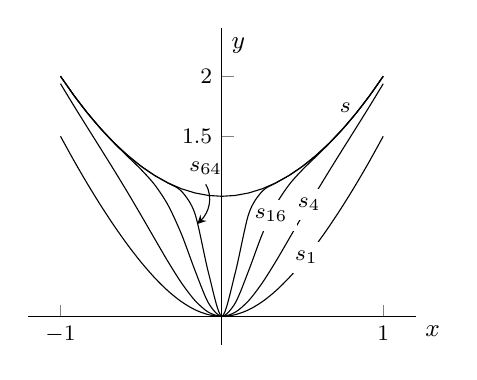
\begin{tikzpicture}
\begin{axis}[small,axis lines*=middle,ymax=2.4,xtick={-1,0,1},xticklabels={$-1$,$0$,$1$},ytick={1.5,2},yticklabels={$1.5$,$2$},xlabel={$x$},ylabel={$y$},xlabel style={at={(current axis.right of origin)},anchor=north west},ylabel style={rotate=-90},ylabel style={at={(current axis.above origin)},anchor=north west}]
\addplot[domain=-1:1,smooth] {1+x^2-1/(1+x^2)^1}node[pos=0.7,fill=white,font=\footnotesize]{$s_1$};
\addplot[domain=-1:1,smooth] {1+x^2-1/(1+x^2)^4}node[pos=0.75,fill=white,font=\footnotesize]{$s_4$};
\addplot[domain=-1:1,smooth] {1+x^2-1/(1+x^2)^16}node[pos=0.7,fill=white,font=\footnotesize]{$s_{16}$};
\addplot[domain=-1:1,smooth] {1+x^2-1/(1+x^2)^64}coordinate[pos=0.33](kA);
\addplot[domain=-1:1] {1+x^2}node[pos=0.9,left,font=\footnotesize]{$s$};
\draw[stealth-] (kA) to [out=45,in=-60](axis cs:-0.1,1.1)node[above,font=\footnotesize]{$s_{64}$};
\end{axis}
\end{tikzpicture}
\caption{مثال \حوالہ{مثال_ٹیلر_عجیب_تسلسل} کے چند جزوی مجموعے}
\label{شکل_مثال_ٹیلر_عجیب_تسلسل}
\end{figure}
\انتہا{مثال}
%==========================

